% Options for packages loaded elsewhere
\PassOptionsToPackage{unicode}{hyperref}
\PassOptionsToPackage{hyphens}{url}
%
\documentclass[
]{article}
\usepackage{lmodern}
\usepackage{amssymb,amsmath}
\usepackage{ifxetex,ifluatex}
\ifnum 0\ifxetex 1\fi\ifluatex 1\fi=0 % if pdftex
  \usepackage[T1]{fontenc}
  \usepackage[utf8]{inputenc}
  \usepackage{textcomp} % provide euro and other symbols
\else % if luatex or xetex
  \usepackage{unicode-math}
  \defaultfontfeatures{Scale=MatchLowercase}
  \defaultfontfeatures[\rmfamily]{Ligatures=TeX,Scale=1}
\fi
% Use upquote if available, for straight quotes in verbatim environments
\IfFileExists{upquote.sty}{\usepackage{upquote}}{}
\IfFileExists{microtype.sty}{% use microtype if available
  \usepackage[]{microtype}
  \UseMicrotypeSet[protrusion]{basicmath} % disable protrusion for tt fonts
}{}
\makeatletter
\@ifundefined{KOMAClassName}{% if non-KOMA class
  \IfFileExists{parskip.sty}{%
    \usepackage{parskip}
  }{% else
    \setlength{\parindent}{0pt}
    \setlength{\parskip}{6pt plus 2pt minus 1pt}}
}{% if KOMA class
  \KOMAoptions{parskip=half}}
\makeatother
\usepackage{xcolor}
\IfFileExists{xurl.sty}{\usepackage{xurl}}{} % add URL line breaks if available
\IfFileExists{bookmark.sty}{\usepackage{bookmark}}{\usepackage{hyperref}}
\hypersetup{
  pdftitle={01 Data Wrangling},
  pdfauthor={Thomas J. Brailey},
  hidelinks,
  pdfcreator={LaTeX via pandoc}}
\urlstyle{same} % disable monospaced font for URLs
\usepackage[margin=1in]{geometry}
\usepackage{color}
\usepackage{fancyvrb}
\newcommand{\VerbBar}{|}
\newcommand{\VERB}{\Verb[commandchars=\\\{\}]}
\DefineVerbatimEnvironment{Highlighting}{Verbatim}{commandchars=\\\{\}}
% Add ',fontsize=\small' for more characters per line
\usepackage{framed}
\definecolor{shadecolor}{RGB}{248,248,248}
\newenvironment{Shaded}{\begin{snugshade}}{\end{snugshade}}
\newcommand{\AlertTok}[1]{\textcolor[rgb]{0.94,0.16,0.16}{#1}}
\newcommand{\AnnotationTok}[1]{\textcolor[rgb]{0.56,0.35,0.01}{\textbf{\textit{#1}}}}
\newcommand{\AttributeTok}[1]{\textcolor[rgb]{0.77,0.63,0.00}{#1}}
\newcommand{\BaseNTok}[1]{\textcolor[rgb]{0.00,0.00,0.81}{#1}}
\newcommand{\BuiltInTok}[1]{#1}
\newcommand{\CharTok}[1]{\textcolor[rgb]{0.31,0.60,0.02}{#1}}
\newcommand{\CommentTok}[1]{\textcolor[rgb]{0.56,0.35,0.01}{\textit{#1}}}
\newcommand{\CommentVarTok}[1]{\textcolor[rgb]{0.56,0.35,0.01}{\textbf{\textit{#1}}}}
\newcommand{\ConstantTok}[1]{\textcolor[rgb]{0.00,0.00,0.00}{#1}}
\newcommand{\ControlFlowTok}[1]{\textcolor[rgb]{0.13,0.29,0.53}{\textbf{#1}}}
\newcommand{\DataTypeTok}[1]{\textcolor[rgb]{0.13,0.29,0.53}{#1}}
\newcommand{\DecValTok}[1]{\textcolor[rgb]{0.00,0.00,0.81}{#1}}
\newcommand{\DocumentationTok}[1]{\textcolor[rgb]{0.56,0.35,0.01}{\textbf{\textit{#1}}}}
\newcommand{\ErrorTok}[1]{\textcolor[rgb]{0.64,0.00,0.00}{\textbf{#1}}}
\newcommand{\ExtensionTok}[1]{#1}
\newcommand{\FloatTok}[1]{\textcolor[rgb]{0.00,0.00,0.81}{#1}}
\newcommand{\FunctionTok}[1]{\textcolor[rgb]{0.00,0.00,0.00}{#1}}
\newcommand{\ImportTok}[1]{#1}
\newcommand{\InformationTok}[1]{\textcolor[rgb]{0.56,0.35,0.01}{\textbf{\textit{#1}}}}
\newcommand{\KeywordTok}[1]{\textcolor[rgb]{0.13,0.29,0.53}{\textbf{#1}}}
\newcommand{\NormalTok}[1]{#1}
\newcommand{\OperatorTok}[1]{\textcolor[rgb]{0.81,0.36,0.00}{\textbf{#1}}}
\newcommand{\OtherTok}[1]{\textcolor[rgb]{0.56,0.35,0.01}{#1}}
\newcommand{\PreprocessorTok}[1]{\textcolor[rgb]{0.56,0.35,0.01}{\textit{#1}}}
\newcommand{\RegionMarkerTok}[1]{#1}
\newcommand{\SpecialCharTok}[1]{\textcolor[rgb]{0.00,0.00,0.00}{#1}}
\newcommand{\SpecialStringTok}[1]{\textcolor[rgb]{0.31,0.60,0.02}{#1}}
\newcommand{\StringTok}[1]{\textcolor[rgb]{0.31,0.60,0.02}{#1}}
\newcommand{\VariableTok}[1]{\textcolor[rgb]{0.00,0.00,0.00}{#1}}
\newcommand{\VerbatimStringTok}[1]{\textcolor[rgb]{0.31,0.60,0.02}{#1}}
\newcommand{\WarningTok}[1]{\textcolor[rgb]{0.56,0.35,0.01}{\textbf{\textit{#1}}}}
\usepackage{graphicx,grffile}
\makeatletter
\def\maxwidth{\ifdim\Gin@nat@width>\linewidth\linewidth\else\Gin@nat@width\fi}
\def\maxheight{\ifdim\Gin@nat@height>\textheight\textheight\else\Gin@nat@height\fi}
\makeatother
% Scale images if necessary, so that they will not overflow the page
% margins by default, and it is still possible to overwrite the defaults
% using explicit options in \includegraphics[width, height, ...]{}
\setkeys{Gin}{width=\maxwidth,height=\maxheight,keepaspectratio}
% Set default figure placement to htbp
\makeatletter
\def\fps@figure{htbp}
\makeatother
\setlength{\emergencystretch}{3em} % prevent overfull lines
\providecommand{\tightlist}{%
  \setlength{\itemsep}{0pt}\setlength{\parskip}{0pt}}
\setcounter{secnumdepth}{-\maxdimen} % remove section numbering

\title{01 Data Wrangling}
\author{Thomas J. Brailey}
\date{29/09/2019}

\begin{document}
\maketitle

{
\setcounter{tocdepth}{2}
\tableofcontents
}
\hypertarget{load-data}{%
\section{Load data}\label{load-data}}

\begin{Shaded}
\begin{Highlighting}[]
\CommentTok{# Set working directory }
\NormalTok{wd <-}\StringTok{ }\KeywordTok{paste0}\NormalTok{(here}\OperatorTok{::}\KeywordTok{here}\NormalTok{(), }\StringTok{'/data/'}\NormalTok{) }

\CommentTok{# Install datasets}
\CommentTok{# Power-sharing-specific datasets}
\NormalTok{idc <-}\StringTok{ }\NormalTok{rio}\OperatorTok{::}\KeywordTok{import}\NormalTok{(}\KeywordTok{paste0}\NormalTok{(wd, }\StringTok{'IDC_country-year_v1_0.RData'}\NormalTok{))}
\NormalTok{dtd <-}\StringTok{ }\NormalTok{rio}\OperatorTok{::}\KeywordTok{import}\NormalTok{(}\KeywordTok{paste0}\NormalTok{(wd,}\StringTok{'Democracy Timeseries Data January 2009 Excel2007.csv'}\NormalTok{))}
\NormalTok{vdem <-}\StringTok{ }\NormalTok{rio}\OperatorTok{::}\KeywordTok{import}\NormalTok{(}\KeywordTok{paste0}\NormalTok{(wd,}\StringTok{"V-Dem-CY+Others-v8.csv"}\NormalTok{))}
\NormalTok{dpi <-}\StringTok{ }\NormalTok{rio}\OperatorTok{::}\KeywordTok{import}\NormalTok{(}\KeywordTok{paste0}\NormalTok{(wd,}\StringTok{'DPI2012.xls'}\NormalTok{))}
\NormalTok{qog_ts <-}\StringTok{ }\NormalTok{rio}\OperatorTok{::}\KeywordTok{import}\NormalTok{(}\KeywordTok{paste0}\NormalTok{(wd,}\StringTok{'qog_std_ts_jan19.csv'}\NormalTok{))}
\NormalTok{ucdp <-}\StringTok{ }\NormalTok{rio}\OperatorTok{::}\KeywordTok{import}\NormalTok{(}\KeywordTok{paste0}\NormalTok{(wd, }\StringTok{"ucdp-prio-acd-191.xlsx"}\NormalTok{))}
\NormalTok{intra <-}\StringTok{ }\NormalTok{rio}\OperatorTok{::}\KeywordTok{import}\NormalTok{(}\KeywordTok{paste0}\NormalTok{(wd, }\StringTok{'annual_onset.dta'}\NormalTok{))}
\NormalTok{p4 <-}\StringTok{ }\NormalTok{rio}\OperatorTok{::}\KeywordTok{import}\NormalTok{(}\KeywordTok{paste0}\NormalTok{(here}\OperatorTok{::}\KeywordTok{here}\NormalTok{(), }\StringTok{"/data/p4v2017.xls"}\NormalTok{))}
\end{Highlighting}
\end{Shaded}

\hypertarget{tidy-datasets}{%
\section{Tidy datasets}\label{tidy-datasets}}

\hypertarget{set-baseline-data}{%
\subsection{Set baseline data}\label{set-baseline-data}}

\begin{Shaded}
\begin{Highlighting}[]
\CommentTok{# Use Strom et al.'s (2017) data as baseline}
\NormalTok{tb <-}\StringTok{ }\NormalTok{idc}

\CommentTok{# Rename unmatched countries}
\NormalTok{tb}\OperatorTok{$}\NormalTok{country[tb}\OperatorTok{$}\NormalTok{country }\OperatorTok{==}\StringTok{ "Cent. Af. Rep."}\NormalTok{] <-}\StringTok{ "Central African Republic"}
\NormalTok{tb}\OperatorTok{$}\NormalTok{country[tb}\OperatorTok{$}\NormalTok{country }\OperatorTok{==}\StringTok{ "Dom. Rep."}\NormalTok{] <-}\StringTok{ "Dominican Republic"}
\NormalTok{tb}\OperatorTok{$}\NormalTok{country[tb}\OperatorTok{$}\NormalTok{country }\OperatorTok{==}\StringTok{ "GDR"}\NormalTok{] <-}\StringTok{ "German Democratic Republic"}
\NormalTok{tb}\OperatorTok{$}\NormalTok{country[tb}\OperatorTok{$}\NormalTok{country }\OperatorTok{==}\StringTok{ "PRC"}\NormalTok{] <-}\StringTok{ "China"}
\NormalTok{tb}\OperatorTok{$}\NormalTok{country[tb}\OperatorTok{$}\NormalTok{country }\OperatorTok{==}\StringTok{ "ROK"}\NormalTok{] <-}\StringTok{ "South Korea"}
\NormalTok{tb}\OperatorTok{$}\NormalTok{country[tb}\OperatorTok{$}\NormalTok{country }\OperatorTok{==}\StringTok{ "S. Africa"}\NormalTok{] <-}\StringTok{ "South Africa"}
\NormalTok{tb}\OperatorTok{$}\NormalTok{country[tb}\OperatorTok{$}\NormalTok{country }\OperatorTok{==}\StringTok{ "Serbia and Montenegro"}\NormalTok{] <-}\StringTok{ "Montenegro"}

\NormalTok{tb <-}\StringTok{ }\NormalTok{tb[}\OperatorTok{!}\KeywordTok{is.na}\NormalTok{(tb}\OperatorTok{$}\NormalTok{country) }\OperatorTok{&}\StringTok{ }\OperatorTok{!}\KeywordTok{is.na}\NormalTok{(tb}\OperatorTok{$}\NormalTok{ifs),]}

\NormalTok{tb}\OperatorTok{$}\NormalTok{cowc <-}\StringTok{ }\NormalTok{countrycode}\OperatorTok{::}\KeywordTok{countrycode}\NormalTok{(tb}\OperatorTok{$}\NormalTok{country, }\StringTok{'country.name'}\NormalTok{, }\StringTok{'cowc'}\NormalTok{)}
\end{Highlighting}
\end{Shaded}

\begin{verbatim}
## Warning in countrycode::countrycode(tb$country, "country.name", "cowc"): Some values were not matched unambiguously: Serbia
\end{verbatim}

\begin{Shaded}
\begin{Highlighting}[]
\NormalTok{tb}\OperatorTok{$}\NormalTok{cown <-}\StringTok{ }\NormalTok{countrycode}\OperatorTok{::}\KeywordTok{countrycode}\NormalTok{(tb}\OperatorTok{$}\NormalTok{country, }\StringTok{'country.name'}\NormalTok{, }\StringTok{'cown'}\NormalTok{)}
\end{Highlighting}
\end{Shaded}

\begin{verbatim}
## Warning in countrycode::countrycode(tb$country, "country.name", "cown"): Some values were not matched unambiguously: Serbia
\end{verbatim}

\begin{Shaded}
\begin{Highlighting}[]
\CommentTok{# Some values were not matched unambiguously: Serbia}

\CommentTok{# Select key variables}
\NormalTok{tb <-}\StringTok{ }\NormalTok{tb }\OperatorTok
\StringTok{  }\NormalTok{dplyr}\OperatorTok{::}\KeywordTok{select}\NormalTok{(country, }
\NormalTok{                cowc, }
\NormalTok{                cown, }
\NormalTok{                year, }
\NormalTok{                ifs, }
\NormalTok{                mveto,}
\NormalTok{                gcman,}
\NormalTok{                gcimp,}
\NormalTok{                auton,}
\NormalTok{                jrevman,}
\NormalTok{                relconstd,}
\NormalTok{                relconstp,}
\NormalTok{                milleg,}
\NormalTok{                partynoethnic,}
\NormalTok{                jtenure,}
\NormalTok{                jconst,}
\NormalTok{                gcseats1,}
\NormalTok{                gcseats2,}
\NormalTok{                gcseats3,}
\NormalTok{                unity,}
\NormalTok{                resman,}
\NormalTok{                resseats,}
\NormalTok{                resseats2,}
\NormalTok{                resseatsimp,}
\NormalTok{                miman,}
\NormalTok{                subtax,}
\NormalTok{                subed,}
\NormalTok{                subpolice,}
\NormalTok{                fedunits,}
\NormalTok{                state,}
\NormalTok{                muni,}
                \OperatorTok{-}\NormalTok{ifs}
\NormalTok{                )}
\end{Highlighting}
\end{Shaded}

\hypertarget{clean-vdem}{%
\subsection{Clean VDEM}\label{clean-vdem}}

\begin{Shaded}
\begin{Highlighting}[]
\CommentTok{# Select key variables}
\NormalTok{vdem_psp_sub <-}\StringTok{ }\NormalTok{vdem }\OperatorTok
\StringTok{  }\NormalTok{dplyr}\OperatorTok{::}\KeywordTok{select}\NormalTok{(country_name, }
\NormalTok{                year, }
\NormalTok{                e_miinterc, }
\NormalTok{                e_Civil_War,}
\NormalTok{                v2elfrfair) }\OperatorTok\StringTok{ }
\StringTok{  }\NormalTok{dplyr}\OperatorTok{::}\KeywordTok{rename}\NormalTok{(}\DataTypeTok{country =}\NormalTok{ country_name)}

\NormalTok{vdem_psp_sub}\OperatorTok{$}\NormalTok{country <-}\StringTok{ }\NormalTok{countrycode}\OperatorTok{::}\KeywordTok{countrycode}\NormalTok{(}
\NormalTok{  vdem_psp_sub}\OperatorTok{$}\NormalTok{country, }\StringTok{'country.name'}\NormalTok{, }\StringTok{'country.name'}
\NormalTok{  )}
\end{Highlighting}
\end{Shaded}

\begin{verbatim}
## Warning in countrycode::countrycode(vdem_psp_sub$country, "country.name", : Some values were not matched unambiguously: Democratic Republic of Vietnam, Republic of Vietnam, São Tomé and Príncipe, Würtemberg
\end{verbatim}

\begin{Shaded}
\begin{Highlighting}[]
\NormalTok{vdem_psp_sub}\OperatorTok{$}\NormalTok{cown <-}\StringTok{ }\NormalTok{countrycode}\OperatorTok{::}\KeywordTok{countrycode}\NormalTok{(}
\NormalTok{  vdem_psp_sub}\OperatorTok{$}\NormalTok{country, }\StringTok{'country.name'}\NormalTok{, }\StringTok{'cown'}
\NormalTok{  )}
\end{Highlighting}
\end{Shaded}

\begin{verbatim}
## Warning in countrycode::countrycode(vdem_psp_sub$country, "country.name", : Some values were not matched unambiguously: Brunswick, Hamburg, Hesse-Darmstadt, Hesse-Kassel, Hong Kong SAR China, Nassau, Oldenburg, Palestinian Territories, Piedmont-Sardinia, Saxe-Weimar-Eisenach, Serbia
\end{verbatim}

\begin{Shaded}
\begin{Highlighting}[]
\NormalTok{vdem_psp_sub}\OperatorTok{$}\NormalTok{cowc <-}\StringTok{ }\NormalTok{countrycode}\OperatorTok{::}\KeywordTok{countrycode}\NormalTok{(}
\NormalTok{  vdem_psp_sub}\OperatorTok{$}\NormalTok{country, }\StringTok{'country.name'}\NormalTok{, }\StringTok{'cowc'}
\NormalTok{  )}
\end{Highlighting}
\end{Shaded}

\begin{verbatim}
## Warning in countrycode::countrycode(vdem_psp_sub$country, "country.name", : Some values were not matched unambiguously: Brunswick, Hamburg, Hesse-Darmstadt, Hesse-Kassel, Hong Kong SAR China, Nassau, Oldenburg, Palestinian Territories, Piedmont-Sardinia, Saxe-Weimar-Eisenach, Serbia
\end{verbatim}

\begin{Shaded}
\begin{Highlighting}[]
\NormalTok{vdem_psp_sub <-}\StringTok{ }\NormalTok{vdem_psp_sub }\OperatorTok
\StringTok{  }\NormalTok{dplyr}\OperatorTok{::}\KeywordTok{select}\NormalTok{(}\OperatorTok{-}\NormalTok{country)}
\end{Highlighting}
\end{Shaded}

\hypertarget{clean-qog}{%
\subsection{Clean QoG}\label{clean-qog}}

\begin{Shaded}
\begin{Highlighting}[]
\CommentTok{# Select key variables and clean.}
\NormalTok{qog_ts_psp_sub <-}\StringTok{ }\NormalTok{qog_ts }\OperatorTok
\StringTok{  }\NormalTok{dplyr}\OperatorTok{::}\KeywordTok{select}\NormalTok{(cname, }
\NormalTok{                year, }
\NormalTok{                fe_etfra,}
\NormalTok{                iaep_ebbp,}
\NormalTok{                gle_gdp,}
\NormalTok{                bti_ci,}
\NormalTok{                cspf_sfi,}
\NormalTok{                gtm_unit,}
\NormalTok{                ccp_hr,}
\NormalTok{                ffp_hr,}
\NormalTok{                iiag_phr,}
\NormalTok{                dpi_housesys,}
\NormalTok{                jw_bicameral,}
\NormalTok{                bti_ig,}
\NormalTok{                vdem_partipdem,}
\NormalTok{                iaep_nr,}
\NormalTok{                bti_sop,}
\NormalTok{                bti_ffe,}
\NormalTok{                gol_est,}
\NormalTok{                gol_mt,}
\NormalTok{                iaep_es,}
\NormalTok{                no_ef,}
\NormalTok{                no_ce,}
\NormalTok{                iaep_eccdt,}
\NormalTok{                iaep_ecdl,}
\NormalTok{                iaep_eml,}
\NormalTok{                iaep_epmf,}
\NormalTok{                iaep_evp,}
\NormalTok{                iaep_lcre,}
\NormalTok{                iaep_lego,}
\NormalTok{                iaep_lrit,}
\NormalTok{                wbgi_pve,}
\NormalTok{                hum_satdem,}
\NormalTok{                hum_supdem,}
\NormalTok{                hum_trust,}
\NormalTok{                wdi_gini,}
\NormalTok{                gle_pop,}
\NormalTok{                al_ethnic,}
\NormalTok{                dpi_auton,}
\NormalTok{                pt_federal}
\NormalTok{  ) }\OperatorTok
\StringTok{  }\NormalTok{dplyr}\OperatorTok{::}\KeywordTok{rename}\NormalTok{(}\DataTypeTok{country =}\NormalTok{ cname)}

\NormalTok{qog_ts_psp_sub}\OperatorTok{$}\NormalTok{country[}
\NormalTok{  qog_ts_psp_sub}\OperatorTok{$}\NormalTok{country }\OperatorTok{==}\StringTok{ "Micronesia"}
\NormalTok{  ] <-}\StringTok{ "Federated States of Micronesia"}
\NormalTok{qog_ts_psp_sub}\OperatorTok{$}\NormalTok{country[}
\NormalTok{  qog_ts_psp_sub}\OperatorTok{$}\NormalTok{country }\OperatorTok{==}\StringTok{ "Serbia and Montenegro"}
\NormalTok{  ] <-}\StringTok{ "Montenegro"}
\NormalTok{qog_ts_psp_sub}\OperatorTok{$}\NormalTok{country <-}\StringTok{ }\NormalTok{countrycode}\OperatorTok{::}\KeywordTok{countrycode}\NormalTok{(}
\NormalTok{  qog_ts_psp_sub}\OperatorTok{$}\NormalTok{country, }\StringTok{'country.name'}\NormalTok{, }\StringTok{'country.name'}
\NormalTok{  )}
\end{Highlighting}
\end{Shaded}

\begin{verbatim}
## Warning in countrycode::countrycode(qog_ts_psp_sub$country, "country.name", : Some values were not matched unambiguously: Tibet
\end{verbatim}

\begin{Shaded}
\begin{Highlighting}[]
\NormalTok{qog_ts_psp_sub}\OperatorTok{$}\NormalTok{cown <-}\StringTok{ }\NormalTok{countrycode}\OperatorTok{::}\KeywordTok{countrycode}\NormalTok{(}
\NormalTok{  qog_ts_psp_sub}\OperatorTok{$}\NormalTok{country, }\StringTok{'country.name'}\NormalTok{, }\StringTok{'cown'}
\NormalTok{  )}
\end{Highlighting}
\end{Shaded}

\begin{verbatim}
## Warning in countrycode::countrycode(qog_ts_psp_sub$country, "country.name", : Some values were not matched unambiguously: Serbia
\end{verbatim}

\begin{Shaded}
\begin{Highlighting}[]
\NormalTok{qog_ts_psp_sub}\OperatorTok{$}\NormalTok{cowc <-}\StringTok{ }\NormalTok{countrycode}\OperatorTok{::}\KeywordTok{countrycode}\NormalTok{(}
\NormalTok{  qog_ts_psp_sub}\OperatorTok{$}\NormalTok{country, }\StringTok{'country.name'}\NormalTok{, }\StringTok{'cowc'}
\NormalTok{  )}
\end{Highlighting}
\end{Shaded}

\begin{verbatim}
## Warning in countrycode::countrycode(qog_ts_psp_sub$country, "country.name", : Some values were not matched unambiguously: Serbia
\end{verbatim}

\begin{Shaded}
\begin{Highlighting}[]
\NormalTok{qog_ts_psp_sub <-}\StringTok{ }\NormalTok{qog_ts_psp_sub }\OperatorTok
\StringTok{  }\NormalTok{dplyr}\OperatorTok{::}\KeywordTok{select}\NormalTok{(}\OperatorTok{-}\NormalTok{country)}
\end{Highlighting}
\end{Shaded}

\hypertarget{clean-dpi}{%
\subsection{Clean DPI}\label{clean-dpi}}

\begin{Shaded}
\begin{Highlighting}[]
\CommentTok{# Select key variables}
\NormalTok{dpi_psp_sub <-}\StringTok{ }\NormalTok{dpi }\OperatorTok
\StringTok{  }\NormalTok{dplyr}\OperatorTok{::}\KeywordTok{select}\NormalTok{(countryname, }
\NormalTok{                year,}
\NormalTok{                system,}
\NormalTok{                author,}
\NormalTok{                pr,}
\NormalTok{                sensys,}
\NormalTok{                eiec}
\NormalTok{                ) }\OperatorTok
\StringTok{  }\NormalTok{dplyr}\OperatorTok{::}\KeywordTok{rename}\NormalTok{(}\DataTypeTok{country =}\NormalTok{ countryname) }\OperatorTok
\StringTok{  }\NormalTok{dplyr}\OperatorTok{::}\KeywordTok{mutate}\NormalTok{(}\DataTypeTok{year =} \KeywordTok{as.numeric}\NormalTok{(year))}

\NormalTok{dpi_psp_sub}\OperatorTok{$}\NormalTok{country[dpi_psp_sub}\OperatorTok{$}\NormalTok{country }\OperatorTok{==}\StringTok{ "Cent. Af. Rep."}\NormalTok{] <-}\StringTok{ "Central African Republic"}
\NormalTok{dpi_psp_sub}\OperatorTok{$}\NormalTok{country[dpi_psp_sub}\OperatorTok{$}\NormalTok{country }\OperatorTok{==}\StringTok{ "Dom. Rep."}\NormalTok{] <-}\StringTok{ "Dominican Republic"}
\NormalTok{dpi_psp_sub}\OperatorTok{$}\NormalTok{country[dpi_psp_sub}\OperatorTok{$}\NormalTok{country }\OperatorTok{==}\StringTok{ "GDR"}\NormalTok{] <-}\StringTok{ "German Democratic Republic"}
\NormalTok{dpi_psp_sub}\OperatorTok{$}\NormalTok{country[dpi_psp_sub}\OperatorTok{$}\NormalTok{country }\OperatorTok{==}\StringTok{ "PRC"}\NormalTok{] <-}\StringTok{ "China"}
\NormalTok{dpi_psp_sub}\OperatorTok{$}\NormalTok{country[dpi_psp_sub}\OperatorTok{$}\NormalTok{country }\OperatorTok{==}\StringTok{ "PRK"}\NormalTok{] <-}\StringTok{ "North Korea"}
\NormalTok{dpi_psp_sub}\OperatorTok{$}\NormalTok{country[dpi_psp_sub}\OperatorTok{$}\NormalTok{country }\OperatorTok{==}\StringTok{ "ROK"}\NormalTok{] <-}\StringTok{ "South Korea"}
\NormalTok{dpi_psp_sub}\OperatorTok{$}\NormalTok{country[dpi_psp_sub}\OperatorTok{$}\NormalTok{country }\OperatorTok{==}\StringTok{ "S. Africa"}\NormalTok{] <-}\StringTok{ "South Africa"}

\NormalTok{dpi_psp_sub}\OperatorTok{$}\NormalTok{country <-}\StringTok{ }\NormalTok{countrycode}\OperatorTok{::}\KeywordTok{countrycode}\NormalTok{(}
\NormalTok{  dpi_psp_sub}\OperatorTok{$}\NormalTok{country, }\StringTok{'country.name'}\NormalTok{, }\StringTok{'country.name'}
\NormalTok{  )}
\NormalTok{dpi_psp_sub}\OperatorTok{$}\NormalTok{cowc <-}\StringTok{ }\NormalTok{countrycode}\OperatorTok{::}\KeywordTok{countrycode}\NormalTok{(}
\NormalTok{  dpi_psp_sub}\OperatorTok{$}\NormalTok{country, }\StringTok{'country.name'}\NormalTok{, }\StringTok{'cowc'}
\NormalTok{  )}
\NormalTok{dpi_psp_sub}\OperatorTok{$}\NormalTok{cown <-}\StringTok{ }\NormalTok{countrycode}\OperatorTok{::}\KeywordTok{countrycode}\NormalTok{(}
\NormalTok{  dpi_psp_sub}\OperatorTok{$}\NormalTok{country, }\StringTok{'country.name'}\NormalTok{, }\StringTok{'cown'}
\NormalTok{  )}

\NormalTok{dpi_psp_sub <-}\StringTok{ }\NormalTok{dpi_psp_sub }\OperatorTok
\StringTok{  }\NormalTok{dplyr}\OperatorTok{::}\KeywordTok{select}\NormalTok{(}\OperatorTok{-}\NormalTok{country)}
\end{Highlighting}
\end{Shaded}

\hypertarget{clean-ucdp}{%
\subsection{Clean UCDP}\label{clean-ucdp}}

\begin{Shaded}
\begin{Highlighting}[]
\NormalTok{ucdp_psp_sub <-}\StringTok{ }\NormalTok{ucdp }\OperatorTok\StringTok{ }
\StringTok{  }\NormalTok{dplyr}\OperatorTok{::}\KeywordTok{select}\NormalTok{(location, year, }
\NormalTok{                side_a, side_b, }
\NormalTok{                territory_name, }
\NormalTok{                intensity_level, }
\NormalTok{                cumulative_intensity, }
\NormalTok{                type_of_conflict) }\OperatorTok
\StringTok{  }\NormalTok{dplyr}\OperatorTok{::}\KeywordTok{filter}\NormalTok{(stringr}\OperatorTok{::}\KeywordTok{str_detect}\NormalTok{(location, }\StringTok{","}\NormalTok{, }\DataTypeTok{negate =} \OtherTok{TRUE}\NormalTok{)) }\OperatorTok
\StringTok{  }\NormalTok{dplyr}\OperatorTok{::}\KeywordTok{rename}\NormalTok{(}\DataTypeTok{country =}\NormalTok{ location)}

\NormalTok{ucdp_psp_sub}\OperatorTok{$}\NormalTok{cowc <-}\StringTok{ }\NormalTok{countrycode}\OperatorTok{::}\KeywordTok{countrycode}\NormalTok{(}
\NormalTok{  ucdp_psp_sub}\OperatorTok{$}\NormalTok{country, }\StringTok{"country.name"}\NormalTok{, }\StringTok{"cowc"}
\NormalTok{  )}
\end{Highlighting}
\end{Shaded}

\begin{verbatim}
## Warning in countrycode::countrycode(ucdp_psp_sub$country, "country.name", : Some values were not matched unambiguously: Hyderabad
\end{verbatim}

\begin{Shaded}
\begin{Highlighting}[]
\NormalTok{ucdp_psp_sub}\OperatorTok{$}\NormalTok{cown <-}\StringTok{ }\NormalTok{countrycode}\OperatorTok{::}\KeywordTok{countrycode}\NormalTok{(}
\NormalTok{  ucdp_psp_sub}\OperatorTok{$}\NormalTok{country, }\StringTok{"country.name"}\NormalTok{, }\StringTok{"cown"}
\NormalTok{  )}
\end{Highlighting}
\end{Shaded}

\begin{verbatim}
## Warning in countrycode::countrycode(ucdp_psp_sub$country, "country.name", : Some values were not matched unambiguously: Hyderabad
\end{verbatim}

\begin{Shaded}
\begin{Highlighting}[]
\NormalTok{ucdp_psp_sub <-}\StringTok{ }\NormalTok{dplyr}\OperatorTok{::}\KeywordTok{select}\NormalTok{(ucdp_psp_sub, }\OperatorTok{-}\NormalTok{country) }
\end{Highlighting}
\end{Shaded}

\hypertarget{clean-prio}{%
\subsection{Clean PRIO}\label{clean-prio}}

\begin{Shaded}
\begin{Highlighting}[]
\NormalTok{intra_psp_sub <-}\StringTok{ }\NormalTok{intra }\OperatorTok
\StringTok{  }\NormalTok{dplyr}\OperatorTok{::}\KeywordTok{select}\NormalTok{(gwno, year, onset2)}

\NormalTok{intra_psp_sub}\OperatorTok{$}\NormalTok{cowc <-}\StringTok{ }\NormalTok{countrycode}\OperatorTok{::}\KeywordTok{countrycode}\NormalTok{(}
\NormalTok{  intra_psp_sub}\OperatorTok{$}\NormalTok{gwno, }\StringTok{'gwn'}\NormalTok{, }\StringTok{'cowc'}
\NormalTok{  )}
\end{Highlighting}
\end{Shaded}

\begin{verbatim}
## Warning in countrycode::countrycode(intra_psp_sub$gwno, "gwn", "cowc"): Some values were not matched unambiguously: 711, 816
\end{verbatim}

\begin{Shaded}
\begin{Highlighting}[]
\NormalTok{intra_psp_sub}\OperatorTok{$}\NormalTok{cown <-}\StringTok{ }\NormalTok{countrycode}\OperatorTok{::}\KeywordTok{countrycode}\NormalTok{(}
\NormalTok{  intra_psp_sub}\OperatorTok{$}\NormalTok{gwno, }\StringTok{'gwn'}\NormalTok{, }\StringTok{'cown'}
\NormalTok{  )}
\end{Highlighting}
\end{Shaded}

\begin{verbatim}
## Warning in countrycode::countrycode(intra_psp_sub$gwno, "gwn", "cown"): Some values were not matched unambiguously: 711, 816
\end{verbatim}

\begin{Shaded}
\begin{Highlighting}[]
\NormalTok{intra_psp_sub <-}\StringTok{ }\NormalTok{intra_psp_sub }\OperatorTok\StringTok{ }\NormalTok{dplyr}\OperatorTok{::}\KeywordTok{select}\NormalTok{(}\OperatorTok{-}\NormalTok{gwno)}
\end{Highlighting}
\end{Shaded}

\hypertarget{clean-polityiv}{%
\subsection{Clean PolityIV}\label{clean-polityiv}}

\begin{Shaded}
\begin{Highlighting}[]
\NormalTok{p4_psp_sub <-}\StringTok{ }\NormalTok{p4 }\OperatorTok
\StringTok{  }\NormalTok{dplyr}\OperatorTok{::}\KeywordTok{select}\NormalTok{(country, year, polity, fragment) }

\NormalTok{p4_psp_sub}\OperatorTok{$}\NormalTok{cowc <-}\StringTok{ }\NormalTok{countrycode}\OperatorTok{::}\KeywordTok{countrycode}\NormalTok{(}
\NormalTok{  p4_psp_sub}\OperatorTok{$}\NormalTok{country, }\StringTok{'country.name'}\NormalTok{, }\StringTok{'cowc'}
\NormalTok{  )}
\end{Highlighting}
\end{Shaded}

\begin{verbatim}
## Warning in countrycode::countrycode(p4_psp_sub$country, "country.name", : Some values were not matched unambiguously: Orange Free State, Prussia, Sardinia, Serbia, Serbia and Montenegro, United Province CA
\end{verbatim}

\begin{Shaded}
\begin{Highlighting}[]
\NormalTok{p4_psp_sub}\OperatorTok{$}\NormalTok{cown <-}\StringTok{ }\NormalTok{countrycode}\OperatorTok{::}\KeywordTok{countrycode}\NormalTok{(}
\NormalTok{  p4_psp_sub}\OperatorTok{$}\NormalTok{country, }\StringTok{'country.name'}\NormalTok{, }\StringTok{'cown'}
\NormalTok{  )}
\end{Highlighting}
\end{Shaded}

\begin{verbatim}
## Warning in countrycode::countrycode(p4_psp_sub$country, "country.name", : Some values were not matched unambiguously: Orange Free State, Prussia, Sardinia, Serbia, Serbia and Montenegro, United Province CA
\end{verbatim}

\begin{Shaded}
\begin{Highlighting}[]
\NormalTok{p4_psp_sub <-}\StringTok{ }\NormalTok{p4_psp_sub }\OperatorTok\StringTok{ }
\StringTok{  }\NormalTok{dplyr}\OperatorTok{::}\KeywordTok{filter}\NormalTok{(}\OperatorTok{!}\KeywordTok{is.na}\NormalTok{(cowc)) }\OperatorTok
\StringTok{  }\NormalTok{dplyr}\OperatorTok{::}\KeywordTok{select}\NormalTok{(}\OperatorTok{-}\NormalTok{country)}
\end{Highlighting}
\end{Shaded}

\hypertarget{clean-rai}{%
\subsection{Clean RAI}\label{clean-rai}}

\begin{Shaded}
\begin{Highlighting}[]
\NormalTok{rai_psp_sub <-}\StringTok{ }\NormalTok{rio}\OperatorTok{::}\KeywordTok{import}\NormalTok{(}\KeywordTok{paste0}\NormalTok{(here}\OperatorTok{::}\KeywordTok{here}\NormalTok{(), }\StringTok{"/data/RAI_country_scores_2015.xlsx"}\NormalTok{)) }\OperatorTok
\StringTok{  }\NormalTok{dplyr}\OperatorTok{::}\KeywordTok{select}\NormalTok{(country_name, year, n_RAI) }\OperatorTok
\StringTok{  }\NormalTok{dplyr}\OperatorTok{::}\KeywordTok{mutate}\NormalTok{(}\DataTypeTok{cown =}\NormalTok{ countrycode}\OperatorTok{::}\KeywordTok{countrycode}\NormalTok{(country_name, }\StringTok{"country.name"}\NormalTok{, }\StringTok{"cown"}\NormalTok{),}
                \DataTypeTok{cowc =}\NormalTok{ countrycode}\OperatorTok{::}\KeywordTok{countrycode}\NormalTok{(cown, }\StringTok{"cown"}\NormalTok{, }\StringTok{"cowc"}\NormalTok{),}
                \DataTypeTok{year =} \KeywordTok{as.numeric}\NormalTok{(year)) }\OperatorTok
\StringTok{  }\NormalTok{dplyr}\OperatorTok{::}\KeywordTok{select}\NormalTok{(cown, cowc, year, n_RAI)}
\end{Highlighting}
\end{Shaded}

\begin{verbatim}
## New names:
## * n_rep -> n_rep...11
## * n_lawmaking -> n_lawmaking...12
## * n_rep -> n_rep...21
## * n_lawmaking -> n_lawmaking...24
\end{verbatim}

\begin{verbatim}
## Warning in countrycode::countrycode(country_name, "country.name", "cown"): Some values were not matched unambiguously: Serbia, Serbia and Montenegro
\end{verbatim}

\hypertarget{clean-epr}{%
\subsection{Clean EPR}\label{clean-epr}}

\begin{Shaded}
\begin{Highlighting}[]
\NormalTok{epr <-}\StringTok{ }\NormalTok{rio}\OperatorTok{::}\KeywordTok{import}\NormalTok{(}\KeywordTok{paste0}\NormalTok{(here}\OperatorTok{::}\KeywordTok{here}\NormalTok{(), }\StringTok{"/data/EPR-2018.1.1.csv"}\NormalTok{)) }\OperatorTok
\StringTok{  }\NormalTok{dplyr}\OperatorTok{::}\KeywordTok{mutate}\NormalTok{(}\DataTypeTok{cown =}\NormalTok{ countrycode}\OperatorTok{::}\KeywordTok{countrycode}\NormalTok{(gwid, }\StringTok{"gwn"}\NormalTok{, }\StringTok{"cown"}\NormalTok{)) }\OperatorTok
\StringTok{  }\NormalTok{dplyr}\OperatorTok{::}\KeywordTok{select}\NormalTok{(cown, from, group, reg_aut) }\OperatorTok
\StringTok{  }\NormalTok{dplyr}\OperatorTok{::}\KeywordTok{rename}\NormalTok{(}\DataTypeTok{year =}\NormalTok{ from) }\OperatorTok\StringTok{ }
\StringTok{  }\NormalTok{dplyr}\OperatorTok{::}\KeywordTok{group_by}\NormalTok{(cown, group) }\OperatorTok
\StringTok{  }\NormalTok{tidyr}\OperatorTok{::}\KeywordTok{complete}\NormalTok{(cown, group, }
                  \DataTypeTok{year =} \DecValTok{1946}\OperatorTok{:}\DecValTok{2017}\NormalTok{, }
                  \DataTypeTok{fill =} \KeywordTok{list}\NormalTok{(}\DataTypeTok{incidents =} \DecValTok{0}\NormalTok{)) }
\end{Highlighting}
\end{Shaded}

\begin{verbatim}
## Warning in countrycode::countrycode(gwid, "gwn", "cown"): Some values were not matched unambiguously: 340, 711, 816
\end{verbatim}

\begin{Shaded}
\begin{Highlighting}[]
\NormalTok{epr_wide <-}\StringTok{ }\NormalTok{epr }\OperatorTok\StringTok{ }
\StringTok{  }\NormalTok{tidyr}\OperatorTok{::}\KeywordTok{pivot_wider}\NormalTok{(}\DataTypeTok{names_from =}\NormalTok{ group, }
                     \DataTypeTok{values_from =}\NormalTok{ reg_aut) }\OperatorTok
\StringTok{  }\NormalTok{dplyr}\OperatorTok{::}\KeywordTok{group_by}\NormalTok{(cown) }

\NormalTok{epr_wide <-}\StringTok{ }\NormalTok{epr_wide }\OperatorTok
\StringTok{  }\NormalTok{tidyr}\OperatorTok{::}\KeywordTok{fill_}\NormalTok{(}\KeywordTok{names}\NormalTok{(epr_wide[,}\DecValTok{2}\OperatorTok{:}\DecValTok{642}\NormalTok{])) }\OperatorTok
\StringTok{  }\NormalTok{dplyr}\OperatorTok{::}\KeywordTok{ungroup}\NormalTok{()}

\NormalTok{epr_wide}\OperatorTok{$}\NormalTok{reg_aut_cont <-}\StringTok{ }\KeywordTok{rowSums}\NormalTok{(epr_wide[,}\DecValTok{3}\OperatorTok{:}\DecValTok{642}\NormalTok{] }\OperatorTok{==}\StringTok{ }\OtherTok{TRUE}\NormalTok{, }\DataTypeTok{na.rm =} \OtherTok{TRUE}\NormalTok{)}

\NormalTok{epr_psp_sub <-}\StringTok{ }\NormalTok{epr_wide }\OperatorTok\StringTok{  }
\StringTok{  }\NormalTok{dplyr}\OperatorTok{::}\KeywordTok{mutate}\NormalTok{(}\DataTypeTok{reg_aut_dum =} \KeywordTok{ifelse}\NormalTok{(reg_aut_cont }\OperatorTok{>=}\StringTok{ }\DecValTok{1}\NormalTok{, }\DecValTok{1}\NormalTok{, }\DecValTok{0}\NormalTok{),}
                \DataTypeTok{cowc =}\NormalTok{ countrycode}\OperatorTok{::}\KeywordTok{countrycode}\NormalTok{(cown, }\StringTok{"cown"}\NormalTok{, }\StringTok{"cowc"}\NormalTok{)) }\OperatorTok
\StringTok{  }\NormalTok{dplyr}\OperatorTok{::}\KeywordTok{select}\NormalTok{(cown, cowc, year, reg_aut_dum, reg_aut_cont)}
\end{Highlighting}
\end{Shaded}

\hypertarget{join-data}{%
\section{Join data}\label{join-data}}

\begin{Shaded}
\begin{Highlighting}[]
\CommentTok{# Join data one-by-one. Check for discrepancies}
\NormalTok{tb_}\DecValTok{2}\NormalTok{ <-}\StringTok{ }\NormalTok{dplyr}\OperatorTok{::}\KeywordTok{left_join}\NormalTok{(tb, qog_ts_psp_sub, }\DataTypeTok{by =} \KeywordTok{c}\NormalTok{(}\StringTok{"cown"}\NormalTok{, }\StringTok{"cowc"}\NormalTok{, }\StringTok{"year"}\NormalTok{))}
\NormalTok{tb_}\DecValTok{3}\NormalTok{ <-}\StringTok{ }\NormalTok{dplyr}\OperatorTok{::}\KeywordTok{left_join}\NormalTok{(tb_}\DecValTok{2}\NormalTok{, dpi_psp_sub, }\DataTypeTok{by =} \KeywordTok{c}\NormalTok{(}\StringTok{"cown"}\NormalTok{, }\StringTok{"cowc"}\NormalTok{, }\StringTok{"year"}\NormalTok{))}
\NormalTok{tb_}\DecValTok{4}\NormalTok{ <-}\StringTok{ }\NormalTok{dplyr}\OperatorTok{::}\KeywordTok{left_join}\NormalTok{(tb_}\DecValTok{3}\NormalTok{, vdem_psp_sub, }\DataTypeTok{by =} \KeywordTok{c}\NormalTok{(}\StringTok{"cown"}\NormalTok{, }\StringTok{"cowc"}\NormalTok{, }\StringTok{"year"}\NormalTok{))}
\NormalTok{tb_}\DecValTok{5}\NormalTok{ <-}\StringTok{ }\NormalTok{dplyr}\OperatorTok{::}\KeywordTok{left_join}\NormalTok{(tb_}\DecValTok{4}\NormalTok{, ucdp_psp_sub, }\DataTypeTok{by =} \KeywordTok{c}\NormalTok{(}\StringTok{"cown"}\NormalTok{, }\StringTok{"cowc"}\NormalTok{, }\StringTok{"year"}\NormalTok{))}
\NormalTok{tb_}\DecValTok{6}\NormalTok{ <-}\StringTok{ }\NormalTok{dplyr}\OperatorTok{::}\KeywordTok{left_join}\NormalTok{(tb_}\DecValTok{5}\NormalTok{, epr_psp_sub, }\DataTypeTok{by =} \KeywordTok{c}\NormalTok{(}\StringTok{"cown"}\NormalTok{, }\StringTok{"cowc"}\NormalTok{, }\StringTok{"year"}\NormalTok{))}
\NormalTok{tb_}\DecValTok{7}\NormalTok{ <-}\StringTok{ }\NormalTok{dplyr}\OperatorTok{::}\KeywordTok{left_join}\NormalTok{(tb_}\DecValTok{6}\NormalTok{, intra_psp_sub, }\DataTypeTok{by =} \KeywordTok{c}\NormalTok{(}\StringTok{"cown"}\NormalTok{, }\StringTok{"cowc"}\NormalTok{, }\StringTok{"year"}\NormalTok{))}
\end{Highlighting}
\end{Shaded}

\begin{verbatim}
## Warning: Column `year` has different attributes on LHS and RHS of join
\end{verbatim}

\begin{Shaded}
\begin{Highlighting}[]
\NormalTok{tb_}\DecValTok{8}\NormalTok{ <-}\StringTok{ }\NormalTok{dplyr}\OperatorTok{::}\KeywordTok{left_join}\NormalTok{(tb_}\DecValTok{7}\NormalTok{, p4_psp_sub, }\DataTypeTok{by =} \KeywordTok{c}\NormalTok{(}\StringTok{"cown"}\NormalTok{, }\StringTok{"cowc"}\NormalTok{, }\StringTok{"year"}\NormalTok{))}
\NormalTok{tb_}\DecValTok{9}\NormalTok{ <-}\StringTok{ }\NormalTok{dplyr}\OperatorTok{::}\KeywordTok{left_join}\NormalTok{(tb_}\DecValTok{8}\NormalTok{, rai_psp_sub, }\DataTypeTok{by =} \KeywordTok{c}\NormalTok{(}\StringTok{"cown"}\NormalTok{, }\StringTok{"cowc"}\NormalTok{, }\StringTok{"year"}\NormalTok{))}

\CommentTok{# Collapse duplicate country/years whie retaining values}
\NormalTok{tb_}\DecValTok{10}\NormalTok{ <-}\StringTok{ }\NormalTok{tb_}\DecValTok{9} \OperatorTok\StringTok{ }
\StringTok{  }\NormalTok{dplyr}\OperatorTok{::}\KeywordTok{group_by}\NormalTok{(country, year) }\OperatorTok
\StringTok{  }\NormalTok{dplyr}\OperatorTok{::}\KeywordTok{summarise_all}\NormalTok{(dplyr}\OperatorTok{::}\KeywordTok{funs}\NormalTok{(dplyr}\OperatorTok{::}\KeywordTok{first}\NormalTok{(}\KeywordTok{na.omit}\NormalTok{(.))))}
\end{Highlighting}
\end{Shaded}

\begin{verbatim}
## Warning: funs() is soft deprecated as of dplyr 0.8.0
## Please use a list of either functions or lambdas: 
## 
##   # Simple named list: 
##   list(mean = mean, median = median)
## 
##   # Auto named with `tibble::lst()`: 
##   tibble::lst(mean, median)
## 
##   # Using lambdas
##   list(~ mean(., trim = .2), ~ median(., na.rm = TRUE))
## This warning is displayed once per session.
\end{verbatim}

\begin{Shaded}
\begin{Highlighting}[]
\CommentTok{# Save data as a .rds file}
\KeywordTok{saveRDS}\NormalTok{(tb_}\DecValTok{10}\NormalTok{, }\KeywordTok{paste0}\NormalTok{(here}\OperatorTok{::}\KeywordTok{here}\NormalTok{(), }\StringTok{'/data/tjbrailey_psp_not_cleaned.rds'}\NormalTok{))}

\CommentTok{# Remove intermediate join files}
\CommentTok{#rm(tb, tb_1, tb_2, tb_3, tb_4, tb_5, tb_6)}
\end{Highlighting}
\end{Shaded}

\hypertarget{visualize-data-before-recoding}{%
\section{Visualize data before
recoding}\label{visualize-data-before-recoding}}

\begin{Shaded}
\begin{Highlighting}[]
\CommentTok{# DataExplorer missingness}
\NormalTok{DataExplorer}\OperatorTok{::}\KeywordTok{plot_missing}\NormalTok{(tb_}\DecValTok{10}\NormalTok{)}
\end{Highlighting}
\end{Shaded}

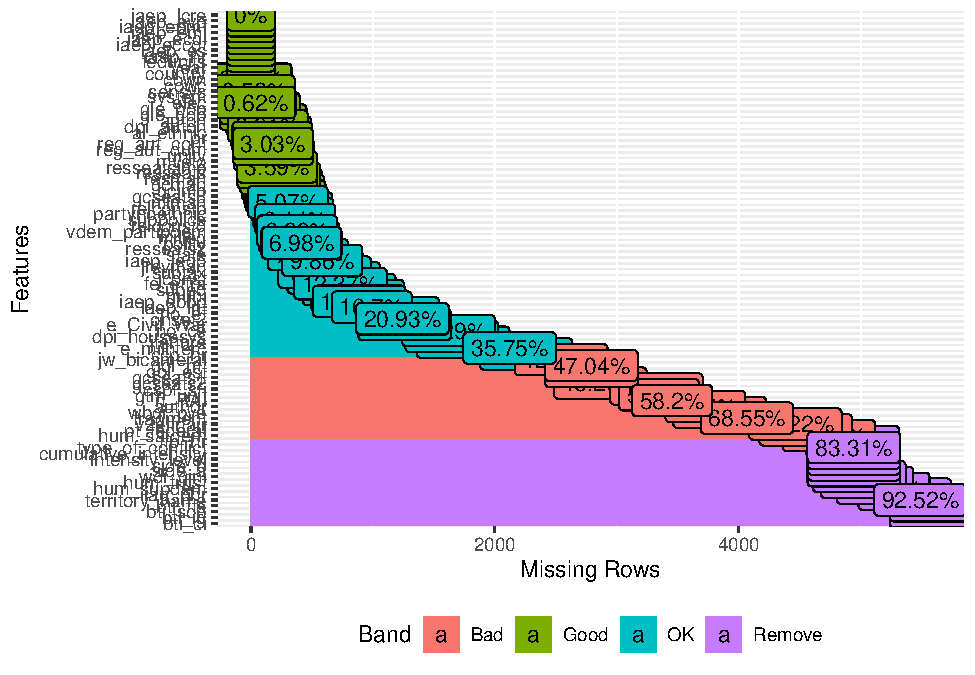
\includegraphics{01_tjbrailey_wrangle_data_files/figure-latex/unnamed-chunk-12-1.pdf}

\begin{Shaded}
\begin{Highlighting}[]
\CommentTok{# Save image}
\KeywordTok{png}\NormalTok{(}\DataTypeTok{file =} \KeywordTok{paste0}\NormalTok{(here}\OperatorTok{::}\KeywordTok{here}\NormalTok{(), }\StringTok{'/vis/tjbrailey_psp_datexp.png'}\NormalTok{),}
    \DataTypeTok{width =} \DecValTok{2000}\NormalTok{,}
    \DataTypeTok{height =} \DecValTok{1000}\NormalTok{)}
\NormalTok{DataExplorer}\OperatorTok{::}\KeywordTok{plot_missing}\NormalTok{(tb_}\DecValTok{10}\NormalTok{)}
\KeywordTok{dev.off}\NormalTok{()}
\end{Highlighting}
\end{Shaded}

\begin{verbatim}
## pdf 
##   2
\end{verbatim}

\begin{Shaded}
\begin{Highlighting}[]
\CommentTok{# DataExplorer variable histograms}
\NormalTok{DataExplorer}\OperatorTok{::}\KeywordTok{plot_histogram}\NormalTok{(tb_}\DecValTok{10}\NormalTok{)}
\end{Highlighting}
\end{Shaded}

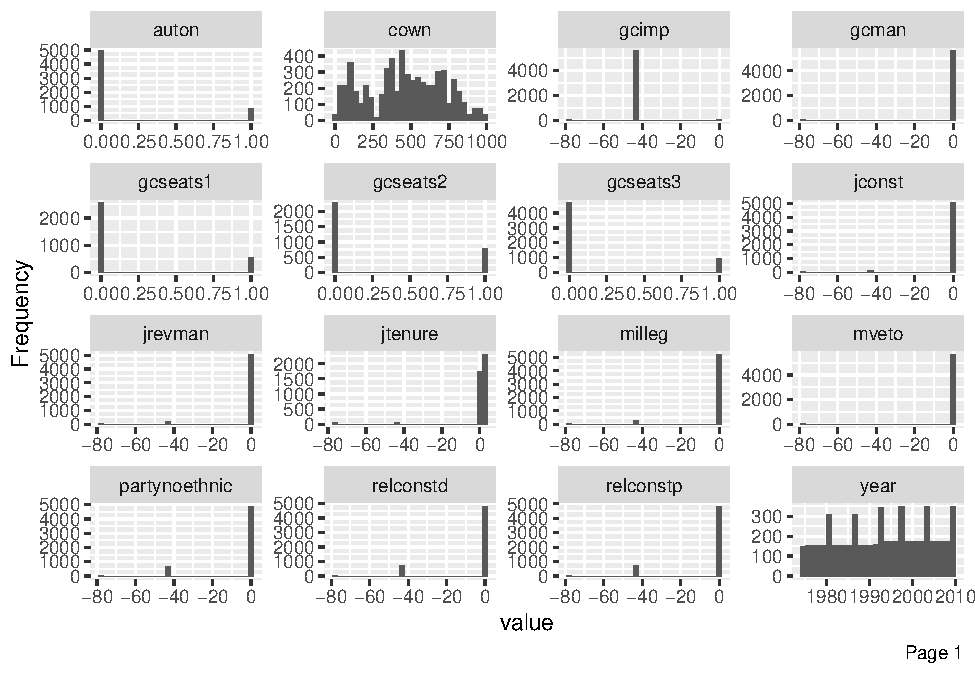
\includegraphics{01_tjbrailey_wrangle_data_files/figure-latex/unnamed-chunk-13-1.pdf}
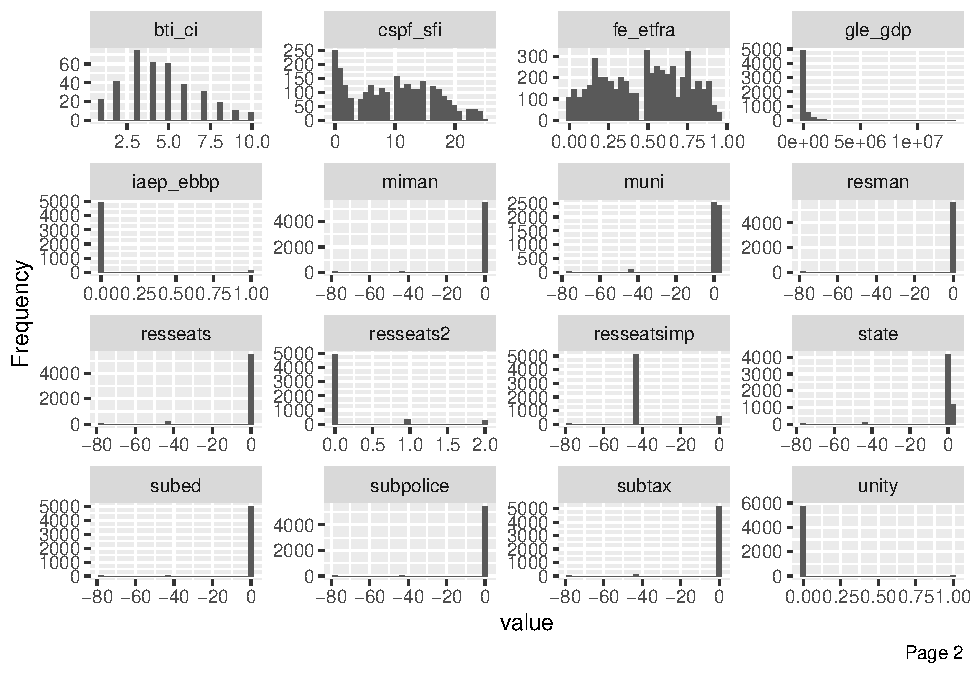
\includegraphics{01_tjbrailey_wrangle_data_files/figure-latex/unnamed-chunk-13-2.pdf}
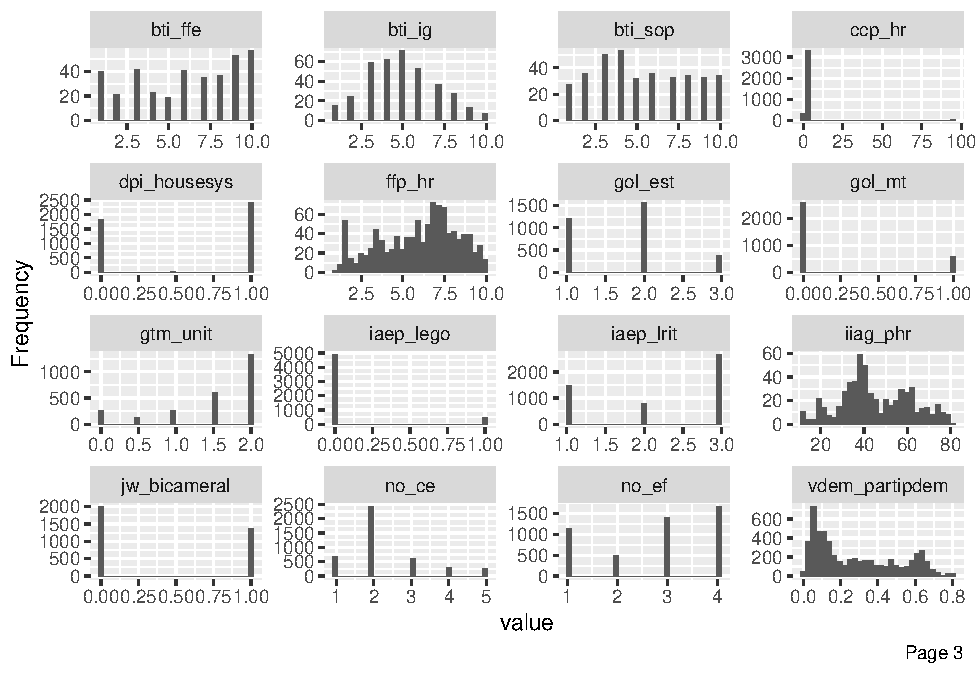
\includegraphics{01_tjbrailey_wrangle_data_files/figure-latex/unnamed-chunk-13-3.pdf}
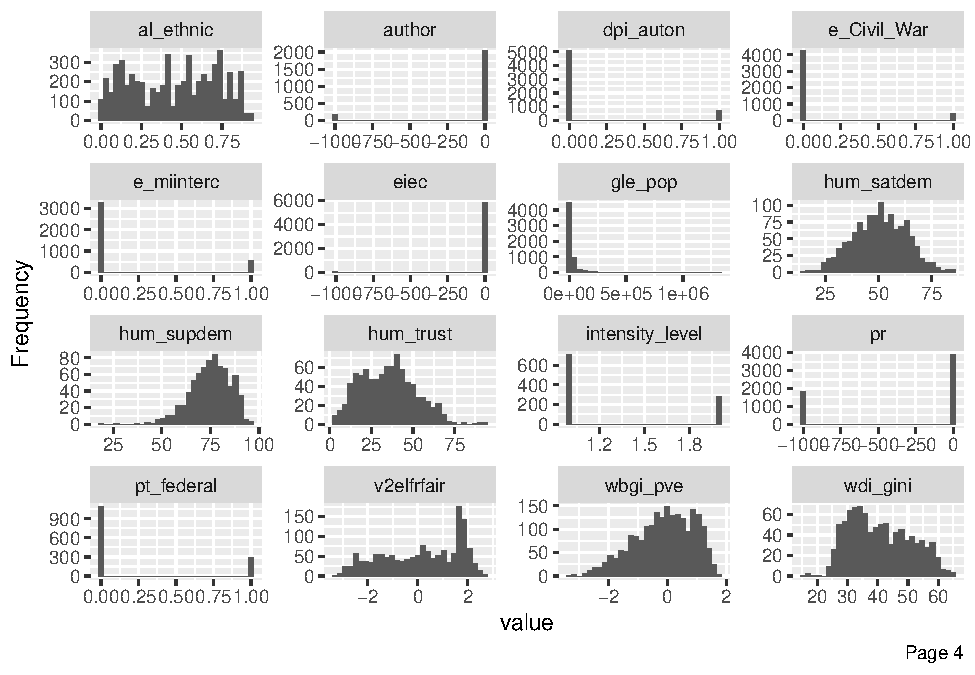
\includegraphics{01_tjbrailey_wrangle_data_files/figure-latex/unnamed-chunk-13-4.pdf}
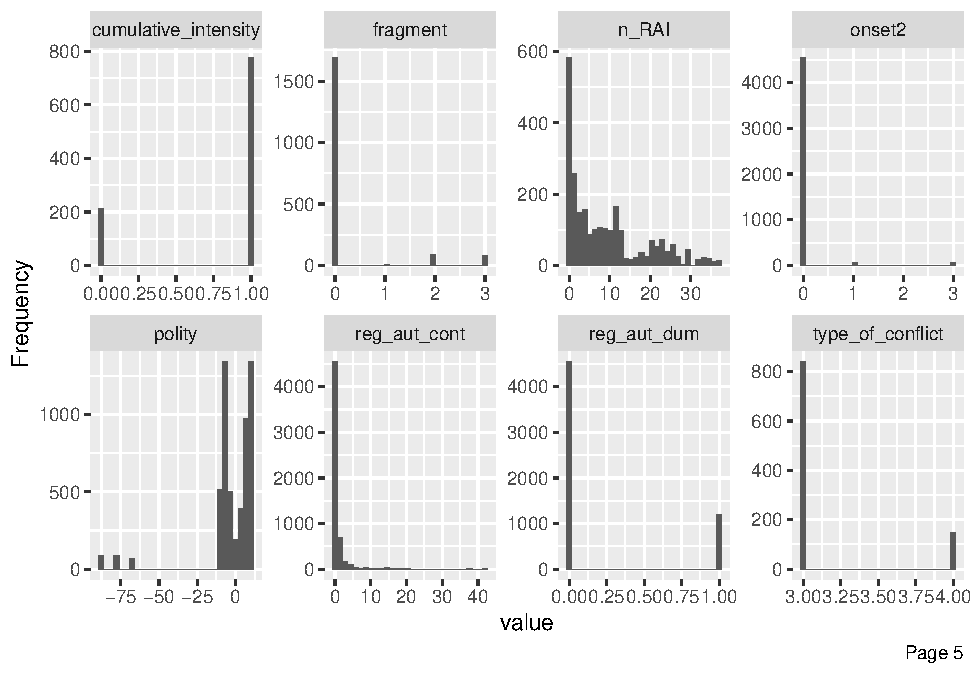
\includegraphics{01_tjbrailey_wrangle_data_files/figure-latex/unnamed-chunk-13-5.pdf}

\begin{Shaded}
\begin{Highlighting}[]
\CommentTok{# Save images}
\KeywordTok{png}\NormalTok{(}\DataTypeTok{file =} \KeywordTok{paste0}\NormalTok{(here}\OperatorTok{::}\KeywordTok{here}\NormalTok{(), }\StringTok{'/vis/tjbrailey_psp_datexp.png'}\NormalTok{),}
    \DataTypeTok{width =} \DecValTok{2000}\NormalTok{,}
    \DataTypeTok{height =} \DecValTok{1000}\NormalTok{)}
\NormalTok{DataExplorer}\OperatorTok{::}\KeywordTok{plot_histogram}\NormalTok{(tb_}\DecValTok{10}\NormalTok{)}
\KeywordTok{dev.off}\NormalTok{()}
\end{Highlighting}
\end{Shaded}

\begin{verbatim}
## pdf 
##   2
\end{verbatim}

\begin{Shaded}
\begin{Highlighting}[]
\CommentTok{# Amelia missingness}
\NormalTok{Amelia}\OperatorTok{::}\KeywordTok{missmap}\NormalTok{(tb_}\DecValTok{10}\NormalTok{)}
\end{Highlighting}
\end{Shaded}

\begin{verbatim}
## Warning: Unknown or uninitialised column: 'arguments'.

## Warning: Unknown or uninitialised column: 'arguments'.
\end{verbatim}

\begin{verbatim}
## Warning: Unknown or uninitialised column: 'imputations'.
\end{verbatim}

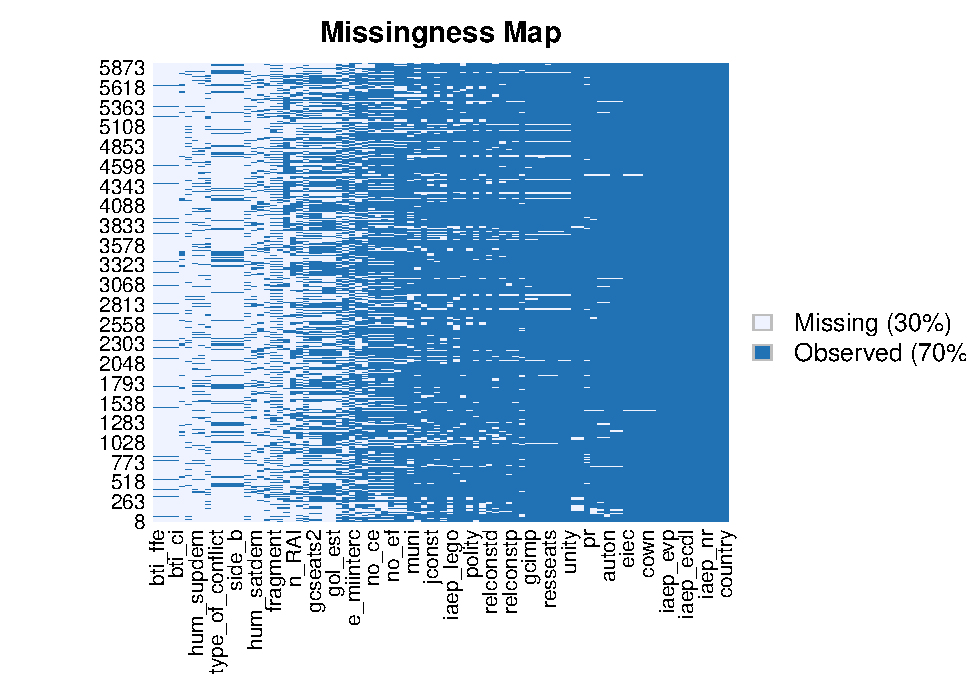
\includegraphics{01_tjbrailey_wrangle_data_files/figure-latex/unnamed-chunk-14-1.pdf}

\begin{Shaded}
\begin{Highlighting}[]
\CommentTok{# Save image}
\KeywordTok{png}\NormalTok{(}\DataTypeTok{file =} \KeywordTok{paste0}\NormalTok{(here}\OperatorTok{::}\KeywordTok{here}\NormalTok{(), }\StringTok{"/vis/tjbrailey_psp_missingness.png"}\NormalTok{),}
    \DataTypeTok{width =} \DecValTok{2000}\NormalTok{, }
    \DataTypeTok{height =} \DecValTok{1000}\NormalTok{)}
\NormalTok{Amelia}\OperatorTok{::}\KeywordTok{missmap}\NormalTok{(tb_}\DecValTok{10}\NormalTok{)}
\end{Highlighting}
\end{Shaded}

\begin{verbatim}
## Warning: Unknown or uninitialised column: 'arguments'.
\end{verbatim}

\begin{verbatim}
## Warning: Unknown or uninitialised column: 'arguments'.
\end{verbatim}

\begin{verbatim}
## Warning: Unknown or uninitialised column: 'imputations'.
\end{verbatim}

\begin{Shaded}
\begin{Highlighting}[]
\KeywordTok{dev.off}\NormalTok{()}
\end{Highlighting}
\end{Shaded}

\begin{verbatim}
## pdf 
##   2
\end{verbatim}

\hypertarget{recode-and-rename-variables}{%
\section{Recode and Rename
Variables}\label{recode-and-rename-variables}}

\begin{Shaded}
\begin{Highlighting}[]
\CommentTok{# Install data}
\NormalTok{psp <-}\StringTok{ }\NormalTok{rio}\OperatorTok{::}\KeywordTok{import}\NormalTok{(}\KeywordTok{paste0}\NormalTok{(here}\OperatorTok{::}\KeywordTok{here}\NormalTok{(), }\StringTok{"/data/tjbrailey_psp_not_cleaned.rds"}\NormalTok{))}

\CommentTok{# Remove codings for NA values}
\NormalTok{psp_na_recode <-}\StringTok{ }\NormalTok{psp}

\NormalTok{psp_na_recode[psp_na_recode }\OperatorTok{==}\StringTok{ "-999"}\NormalTok{] <-}\StringTok{ }\OtherTok{NA}

\NormalTok{psp_na_recode[psp_na_recode }\OperatorTok{==}\StringTok{ "-44"}\NormalTok{] <-}\StringTok{ }\OtherTok{NA}

\NormalTok{psp_na_recode[psp_na_recode }\OperatorTok{==}\StringTok{ "-66"}\NormalTok{] <-}\StringTok{ }\OtherTok{NA}
\NormalTok{psp_na_recode[psp_na_recode }\OperatorTok{==}\StringTok{ "-77"}\NormalTok{] <-}\StringTok{ }\OtherTok{NA}
\NormalTok{psp_na_recode[psp_na_recode }\OperatorTok{==}\StringTok{ "-88"}\NormalTok{] <-}\StringTok{ }\OtherTok{NA}
\NormalTok{psp_na_recode}\OperatorTok{$}\NormalTok{ccp_hr[psp_na_recode}\OperatorTok{$}\NormalTok{ccp_hr }\OperatorTok{==}\StringTok{ "96"}\NormalTok{] <-}\StringTok{ }\DecValTok{3}

\NormalTok{psp_na_recode[psp_na_recode }\OperatorTok{==}\StringTok{ ".a"}\NormalTok{] <-}\StringTok{ }\OtherTok{NA}
\NormalTok{psp_na_recode[psp_na_recode }\OperatorTok{==}\StringTok{ ".b"}\NormalTok{] <-}\StringTok{ }\OtherTok{NA}
\NormalTok{psp_na_recode[psp_na_recode }\OperatorTok{==}\StringTok{ ".e"}\NormalTok{] <-}\StringTok{ }\OtherTok{NA}

\CommentTok{# Rename variables}
\NormalTok{psp_rename <-}\StringTok{ }\NormalTok{psp_na_recode}

\NormalTok{psp_rename <-}\StringTok{ }\NormalTok{psp_rename }\OperatorTok
\StringTok{  }\NormalTok{dplyr}\OperatorTok{::}\KeywordTok{rename}\NormalTok{(}\DataTypeTok{idc_mveto =}\NormalTok{ mveto,}
                \DataTypeTok{idc_gcman =}\NormalTok{ gcman,}
                \DataTypeTok{idc_gcimp =}\NormalTok{ gcimp,}
                \DataTypeTok{idc_auton =}\NormalTok{ auton,}
                \DataTypeTok{idc_jrevman =}\NormalTok{ jrevman,}
                \DataTypeTok{idc_relconstd =}\NormalTok{ relconstd,}
                \DataTypeTok{idc_relconstp =}\NormalTok{ relconstp,}
                \DataTypeTok{idc_milleg =}\NormalTok{ milleg,}
                \DataTypeTok{idc_partynoethnic =}\NormalTok{ partynoethnic,}
                \DataTypeTok{idc_jtenure =}\NormalTok{ jtenure,}
                \DataTypeTok{idc_jconst =}\NormalTok{ jconst,}
                \DataTypeTok{idc_gcseats1 =}\NormalTok{ gcseats1,}
                \DataTypeTok{idc_gcseats2 =}\NormalTok{ gcseats2,}
                \DataTypeTok{idc_gcseats3 =}\NormalTok{ gcseats3,}
                \DataTypeTok{idc_unity =}\NormalTok{ unity,}
                \DataTypeTok{idc_resman =}\NormalTok{ resman,}
                \DataTypeTok{idc_resseats =}\NormalTok{ resseats,}
                \DataTypeTok{idc_resseats2 =}\NormalTok{ resseats2,}
                \DataTypeTok{idc_resseatsimp =}\NormalTok{ resseatsimp,}
                \DataTypeTok{idc_miman =}\NormalTok{ miman, }
                \DataTypeTok{idc_subtax =}\NormalTok{ subtax, }
                \DataTypeTok{idc_subed =}\NormalTok{ subed, }
                \DataTypeTok{idc_subpolice =}\NormalTok{ subpolice,}
                \DataTypeTok{idc_state =}\NormalTok{ state,}
                \DataTypeTok{idc_muni =}\NormalTok{ muni,}
                \DataTypeTok{idc_fedunits =}\NormalTok{ fedunits,}
                
                \DataTypeTok{qog_fe_etfra =}\NormalTok{ fe_etfra,}
                \DataTypeTok{qog_iaep_ebbp =}\NormalTok{ iaep_ebbp,}
                \DataTypeTok{qog_gle_gdp =}\NormalTok{ gle_gdp,}
                \DataTypeTok{qog_bti_ci =}\NormalTok{ bti_ci,}
                \DataTypeTok{qog_cspf_sfi =}\NormalTok{ cspf_sfi,}
                \DataTypeTok{qog_gtm_unit =}\NormalTok{ gtm_unit,}
                \DataTypeTok{qog_ccp_hr =}\NormalTok{ ccp_hr,}
                \DataTypeTok{qog_ffp_hr =}\NormalTok{ ffp_hr, }
                \DataTypeTok{qog_iiag_phr =}\NormalTok{ iiag_phr,}
                \DataTypeTok{qog_dpi_housesys =}\NormalTok{ dpi_housesys,}
                \DataTypeTok{qog_jw_bicameral =}\NormalTok{ jw_bicameral,}
                \DataTypeTok{qog_bti_ig =}\NormalTok{ bti_ig, }
                \DataTypeTok{qog_vdem_partipdem =}\NormalTok{ vdem_partipdem,}
                \DataTypeTok{qog_iaep_nr =}\NormalTok{ iaep_nr,}
                \DataTypeTok{qog_bti_sop =}\NormalTok{ bti_sop,}
                \DataTypeTok{qog_gol_est =}\NormalTok{ gol_est,}
                \DataTypeTok{qog_gol_mt =}\NormalTok{ gol_mt,}
                \DataTypeTok{qog_iaep_es =}\NormalTok{ iaep_es,}
                \DataTypeTok{qog_no_ef =}\NormalTok{ no_ef,}
                \DataTypeTok{qog_no_ce =}\NormalTok{ no_ce,}
                \DataTypeTok{qog_iaep_eccdt =}\NormalTok{ iaep_eccdt,}
                \DataTypeTok{qog_iaep_ecdl =}\NormalTok{ iaep_ecdl,}
                \DataTypeTok{qog_iaep_eml =}\NormalTok{ iaep_eml,}
                \DataTypeTok{qog_iaep_epmf =}\NormalTok{ iaep_epmf,}
                \DataTypeTok{qog_iaep_evp =}\NormalTok{ iaep_evp,}
                \DataTypeTok{qog_iaep_lcre =}\NormalTok{ iaep_lcre,}
                \DataTypeTok{qog_iaep_lego =}\NormalTok{ iaep_lego,}
                \DataTypeTok{qog_iaep_lrit =}\NormalTok{ iaep_lrit,}
                \DataTypeTok{qog_wbgi_pve =}\NormalTok{ wbgi_pve,}
                \DataTypeTok{qog_hum_satdem =}\NormalTok{ hum_satdem,}
                \DataTypeTok{qog_hum_supdem =}\NormalTok{ hum_supdem,}
                \DataTypeTok{qog_hum_trust =}\NormalTok{ hum_trust,}
                \DataTypeTok{qog_wdi_gini =}\NormalTok{ wdi_gini,}
                \DataTypeTok{qog_gle_pop =}\NormalTok{ gle_pop,}
                \DataTypeTok{qog_al_ethnic =}\NormalTok{ al_ethnic,}
                \DataTypeTok{qog_pt_federal =}\NormalTok{ pt_federal,}
                
                \DataTypeTok{dpi_system =}\NormalTok{ system,}
                \DataTypeTok{dpi_author =}\NormalTok{ author,}
                \DataTypeTok{dpi_pr =}\NormalTok{ pr,}
                \DataTypeTok{dpi_sensys =}\NormalTok{ sensys,}
                \DataTypeTok{dpi_eiec =}\NormalTok{ eiec,}
                
                \DataTypeTok{vdem_e_miinterc =}\NormalTok{ e_miinterc, }
                \DataTypeTok{vdem_e_civil_war =}\NormalTok{ e_Civil_War,}
                
                \DataTypeTok{ucdp_side_a =}\NormalTok{ side_a,}
                \DataTypeTok{ucdp_side_b =}\NormalTok{ side_b,}
                \DataTypeTok{ucdp_territory_name =}\NormalTok{ territory_name,}
                \DataTypeTok{ucdp_intensity_level =}\NormalTok{ intensity_level,}
                \DataTypeTok{ucdp_type_of_conflict =}\NormalTok{ type_of_conflict, }
                \DataTypeTok{ucdp_cumulative_intensity =}\NormalTok{ cumulative_intensity,}
                
                \DataTypeTok{prio_onset =}\NormalTok{ onset2,}
                
                \DataTypeTok{polity4_polity_score =}\NormalTok{ polity,}
                \DataTypeTok{polity4_fragment =}\NormalTok{ fragment,}
                
                \DataTypeTok{epr_reg_aut_dum =}\NormalTok{ reg_aut_dum,}
                \DataTypeTok{epr_reg_aut_cont =}\NormalTok{ reg_aut_cont,}
                
                \DataTypeTok{rai_n_RAI =}\NormalTok{ n_RAI}
\NormalTok{                ) }\OperatorTok\StringTok{ }
\StringTok{  }
\StringTok{  }\CommentTok{# Fill out remaining variables}
\StringTok{  }\NormalTok{dplyr}\OperatorTok{::}\KeywordTok{group_by}\NormalTok{(country) }\OperatorTok\StringTok{ }
\StringTok{  }\NormalTok{tidyr}\OperatorTok{::}\KeywordTok{fill}\NormalTok{(qog_wdi_gini, }
\NormalTok{              qog_wbgi_pve, }
\NormalTok{              qog_hum_satdem,}
\NormalTok{              qog_hum_supdem, }
\NormalTok{              qog_hum_trust,}
\NormalTok{              bti_ffe,}
\NormalTok{              v2elfrfair) }

\KeywordTok{variable.names}\NormalTok{(psp_rename)}
\end{Highlighting}
\end{Shaded}

\begin{verbatim}
##  [1] "country"                   "year"                     
##  [3] "cowc"                      "cown"                     
##  [5] "idc_mveto"                 "idc_gcman"                
##  [7] "idc_gcimp"                 "idc_auton"                
##  [9] "idc_jrevman"               "idc_relconstd"            
## [11] "idc_relconstp"             "idc_milleg"               
## [13] "idc_partynoethnic"         "idc_jtenure"              
## [15] "idc_jconst"                "idc_gcseats1"             
## [17] "idc_gcseats2"              "idc_gcseats3"             
## [19] "idc_unity"                 "idc_resman"               
## [21] "idc_resseats"              "idc_resseats2"            
## [23] "idc_resseatsimp"           "idc_miman"                
## [25] "idc_subtax"                "idc_subed"                
## [27] "idc_subpolice"             "idc_fedunits"             
## [29] "idc_state"                 "idc_muni"                 
## [31] "qog_fe_etfra"              "qog_iaep_ebbp"            
## [33] "qog_gle_gdp"               "qog_bti_ci"               
## [35] "qog_cspf_sfi"              "qog_gtm_unit"             
## [37] "qog_ccp_hr"                "qog_ffp_hr"               
## [39] "qog_iiag_phr"              "qog_dpi_housesys"         
## [41] "qog_jw_bicameral"          "qog_bti_ig"               
## [43] "qog_vdem_partipdem"        "qog_iaep_nr"              
## [45] "qog_bti_sop"               "bti_ffe"                  
## [47] "qog_gol_est"               "qog_gol_mt"               
## [49] "qog_iaep_es"               "qog_no_ef"                
## [51] "qog_no_ce"                 "qog_iaep_eccdt"           
## [53] "qog_iaep_ecdl"             "qog_iaep_eml"             
## [55] "qog_iaep_epmf"             "qog_iaep_evp"             
## [57] "qog_iaep_lcre"             "qog_iaep_lego"            
## [59] "qog_iaep_lrit"             "qog_wbgi_pve"             
## [61] "qog_hum_satdem"            "qog_hum_supdem"           
## [63] "qog_hum_trust"             "qog_wdi_gini"             
## [65] "qog_gle_pop"               "qog_al_ethnic"            
## [67] "dpi_auton"                 "qog_pt_federal"           
## [69] "dpi_system"                "dpi_author"               
## [71] "dpi_pr"                    "dpi_sensys"               
## [73] "dpi_eiec"                  "vdem_e_miinterc"          
## [75] "vdem_e_civil_war"          "v2elfrfair"               
## [77] "ucdp_side_a"               "ucdp_side_b"              
## [79] "ucdp_territory_name"       "ucdp_intensity_level"     
## [81] "ucdp_cumulative_intensity" "ucdp_type_of_conflict"    
## [83] "epr_reg_aut_dum"           "epr_reg_aut_cont"         
## [85] "prio_onset"                "polity4_polity_score"     
## [87] "polity4_fragment"          "rai_n_RAI"
\end{verbatim}

\hypertarget{additional-variables}{%
\section{Additional variables}\label{additional-variables}}

\begin{Shaded}
\begin{Highlighting}[]
\NormalTok{psp_add_bin <-}\StringTok{ }\NormalTok{psp_rename }\OperatorTok
\StringTok{  }
\StringTok{  }\CommentTok{# Other provisions}
\StringTok{  }\NormalTok{dplyr}\OperatorTok{::}\KeywordTok{mutate}\NormalTok{(}\DataTypeTok{tb_other_provis =} \KeywordTok{ifelse}\NormalTok{(idc_mveto }\OperatorTok{==}\StringTok{ }\DecValTok{1}\OperatorTok{|}
\StringTok{                                      }\NormalTok{idc_gcman }\OperatorTok{==}\StringTok{ }\DecValTok{1} \OperatorTok{|}
\StringTok{                                        }\NormalTok{idc_gcimp }\OperatorTok{==}\StringTok{ }\DecValTok{1} \OperatorTok{|}
\StringTok{                                        }\NormalTok{dpi_pr }\OperatorTok{==}\StringTok{ }\DecValTok{1}\NormalTok{, }\DecValTok{1}\NormalTok{, }\DecValTok{0}\NormalTok{),}
  \DataTypeTok{tb_other_provis =} \KeywordTok{ifelse}\NormalTok{(}\KeywordTok{is.na}\NormalTok{(tb_other_provis), }\DecValTok{0}\NormalTok{, tb_other_provis)) }\OperatorTok
\StringTok{  }
\StringTok{  }\CommentTok{# Alternative measure of autonomy}
\StringTok{  }\NormalTok{dplyr}\OperatorTok{::}\KeywordTok{mutate}\NormalTok{(}\DataTypeTok{tb_aut =} \KeywordTok{ifelse}\NormalTok{(idc_subtax }\OperatorTok{==}\StringTok{ }\DecValTok{1} \OperatorTok{|}\StringTok{ }
\StringTok{                                  }\NormalTok{idc_subed }\OperatorTok{==}\StringTok{ }\DecValTok{1} \OperatorTok{|}
\StringTok{                                  }\NormalTok{idc_subpolice }\OperatorTok{==}\StringTok{ }\DecValTok{1}\NormalTok{, }\DecValTok{1}\NormalTok{, }\DecValTok{0}\NormalTok{)) }\OperatorTok
\StringTok{  }\NormalTok{dplyr}\OperatorTok{::}\KeywordTok{group_by}\NormalTok{(ucdp_side_a, ucdp_side_b) }\OperatorTok\StringTok{ }
\StringTok{  }
\StringTok{  }\CommentTok{# Length of conflict}
\StringTok{  }\NormalTok{dplyr}\OperatorTok{::}\KeywordTok{mutate}\NormalTok{(}\DataTypeTok{tb_conflict_length =} \KeywordTok{sum}\NormalTok{(}
    \KeywordTok{length}\NormalTok{(ucdp_cumulative_intensity), }\DataTypeTok{na.rm =}\NormalTok{ T)}
\NormalTok{    ) }\OperatorTok
\StringTok{  }\NormalTok{dplyr}\OperatorTok{::}\KeywordTok{ungroup}\NormalTok{()}
  
\NormalTok{psp_add_bin}\OperatorTok{$}\NormalTok{tb_conflict_length[psp_add_bin}\OperatorTok{$}\NormalTok{tb_conflict_length }\OperatorTok{==}\StringTok{ }\DecValTok{4943}\NormalTok{] <-}\StringTok{ }\OtherTok{NA}
\end{Highlighting}
\end{Shaded}

\hypertarget{save-final-data}{%
\section{Save final data}\label{save-final-data}}

\begin{Shaded}
\begin{Highlighting}[]
\CommentTok{# Save as a .csv file }
\CommentTok{#write.csv(psp_add_bin, file = paste0(here::here(), "/data/tjbrailey_psp_clean.csv"))}
\end{Highlighting}
\end{Shaded}

\hypertarget{visualize-after-recoding}{%
\section{Visualize after recoding}\label{visualize-after-recoding}}

\begin{Shaded}
\begin{Highlighting}[]
\NormalTok{DataExplorer}\OperatorTok{::}\KeywordTok{plot_missing}\NormalTok{(psp_add_bin)}
\end{Highlighting}
\end{Shaded}

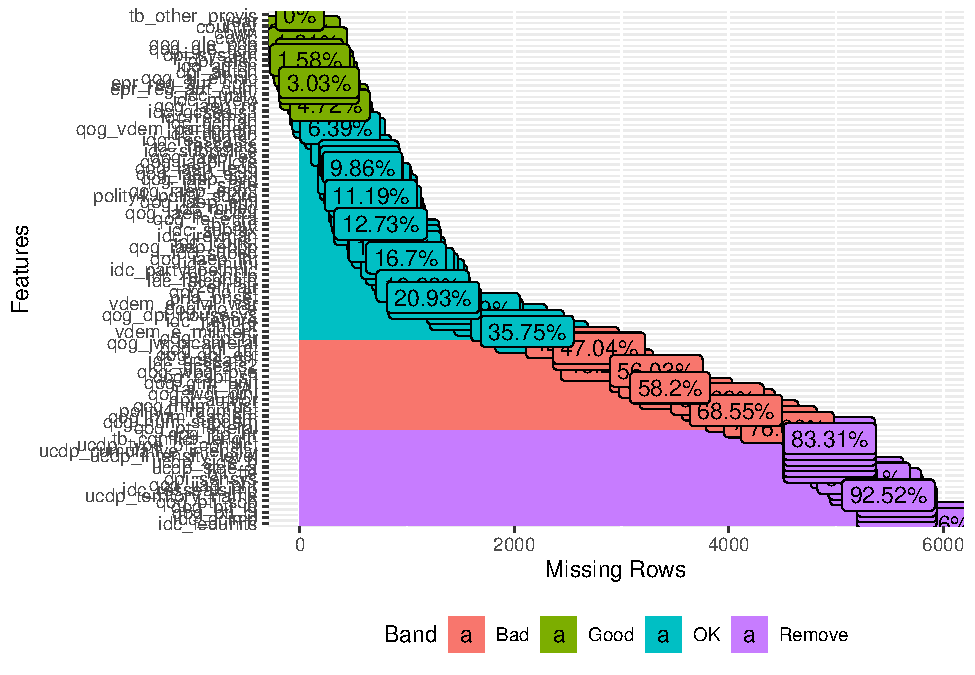
\includegraphics{01_tjbrailey_wrangle_data_files/figure-latex/unnamed-chunk-18-1.pdf}

\begin{Shaded}
\begin{Highlighting}[]
\NormalTok{DataExplorer}\OperatorTok{::}\KeywordTok{plot_histogram}\NormalTok{(psp_add_bin)}
\end{Highlighting}
\end{Shaded}

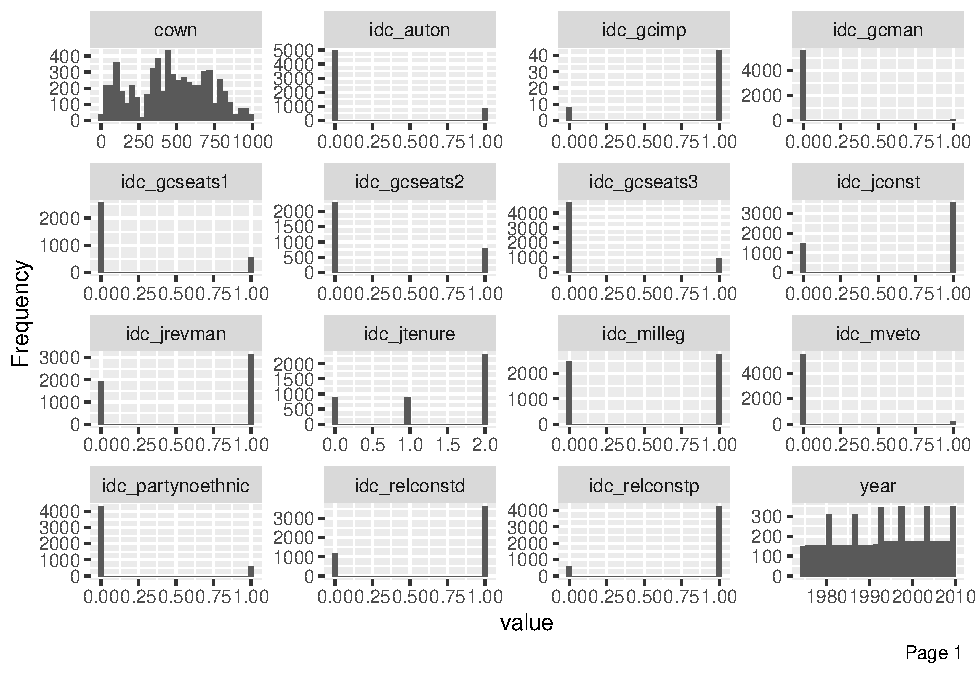
\includegraphics{01_tjbrailey_wrangle_data_files/figure-latex/unnamed-chunk-19-1.pdf}
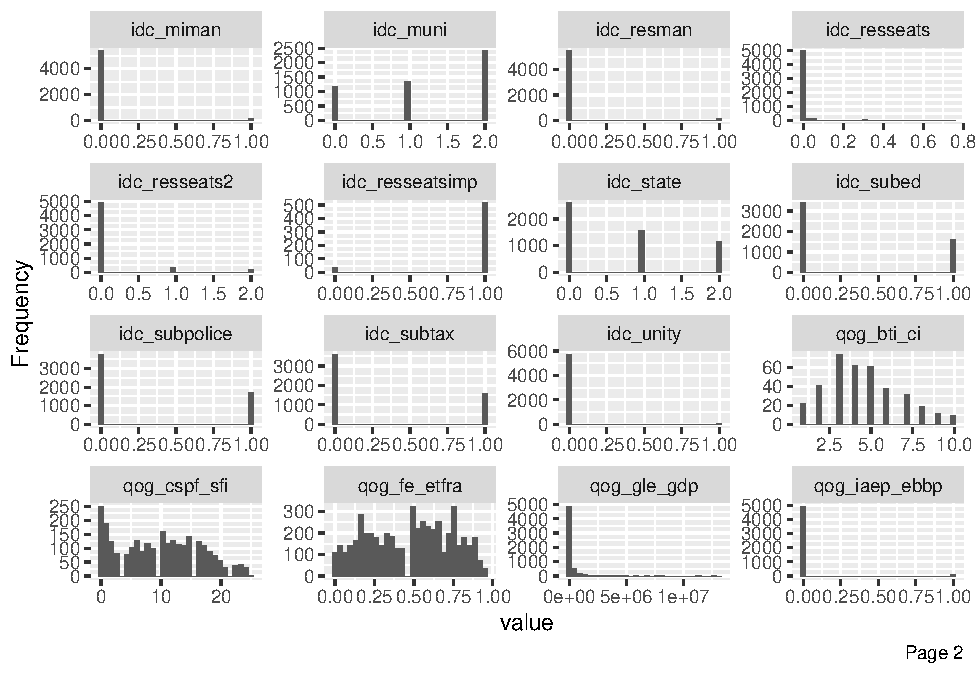
\includegraphics{01_tjbrailey_wrangle_data_files/figure-latex/unnamed-chunk-19-2.pdf}
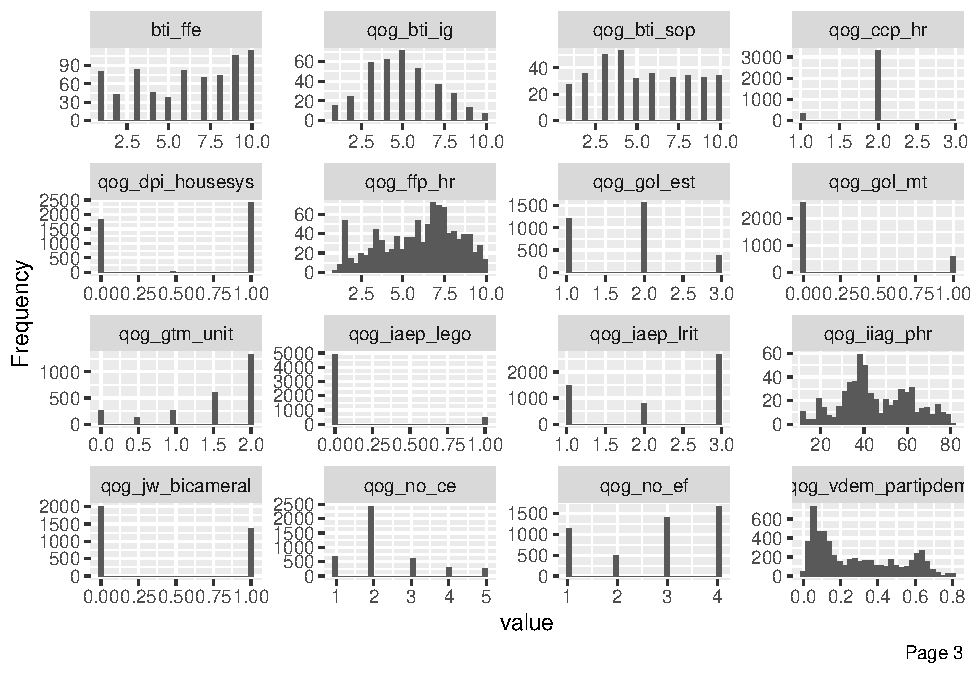
\includegraphics{01_tjbrailey_wrangle_data_files/figure-latex/unnamed-chunk-19-3.pdf}
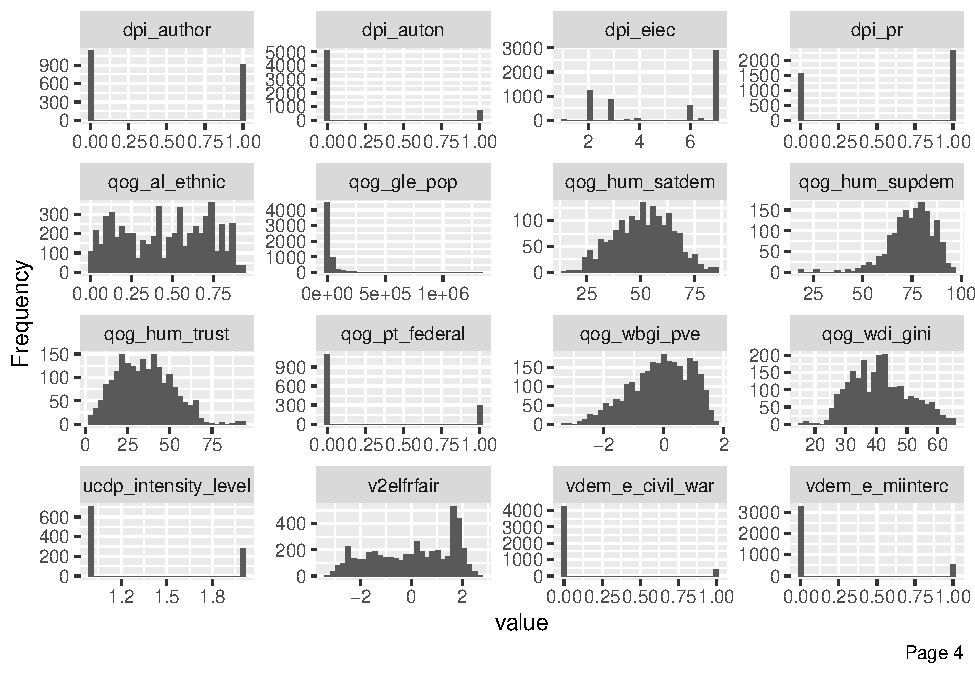
\includegraphics{01_tjbrailey_wrangle_data_files/figure-latex/unnamed-chunk-19-4.pdf}
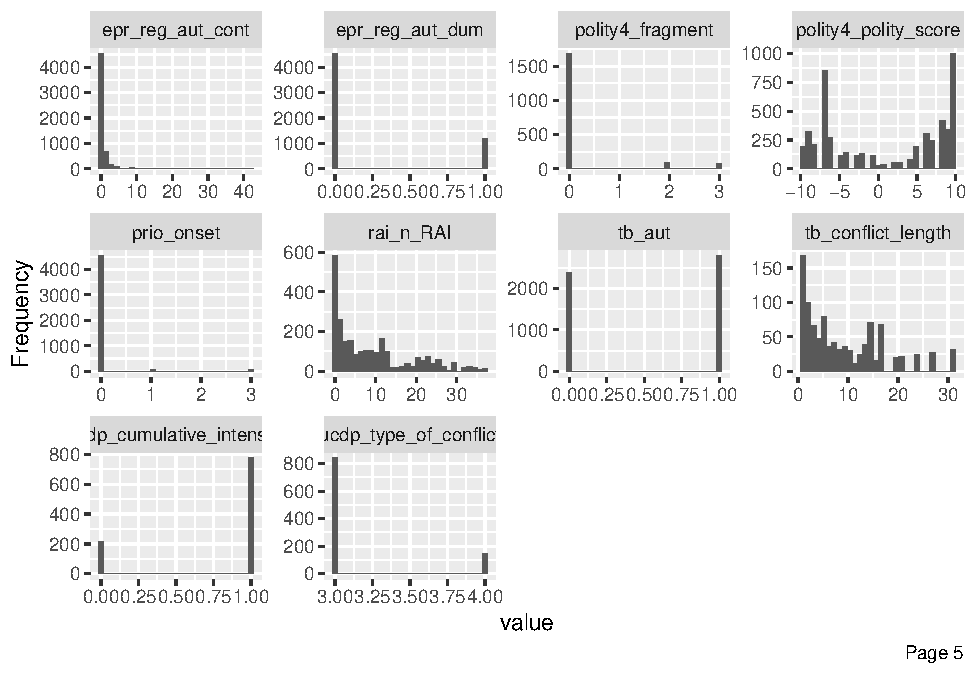
\includegraphics{01_tjbrailey_wrangle_data_files/figure-latex/unnamed-chunk-19-5.pdf}

\begin{Shaded}
\begin{Highlighting}[]
\NormalTok{Amelia}\OperatorTok{::}\KeywordTok{missmap}\NormalTok{(psp_add_bin)}
\end{Highlighting}
\end{Shaded}

\begin{verbatim}
## Warning: Unknown or uninitialised column: 'arguments'.

## Warning: Unknown or uninitialised column: 'arguments'.
\end{verbatim}

\begin{verbatim}
## Warning: Unknown or uninitialised column: 'imputations'.
\end{verbatim}

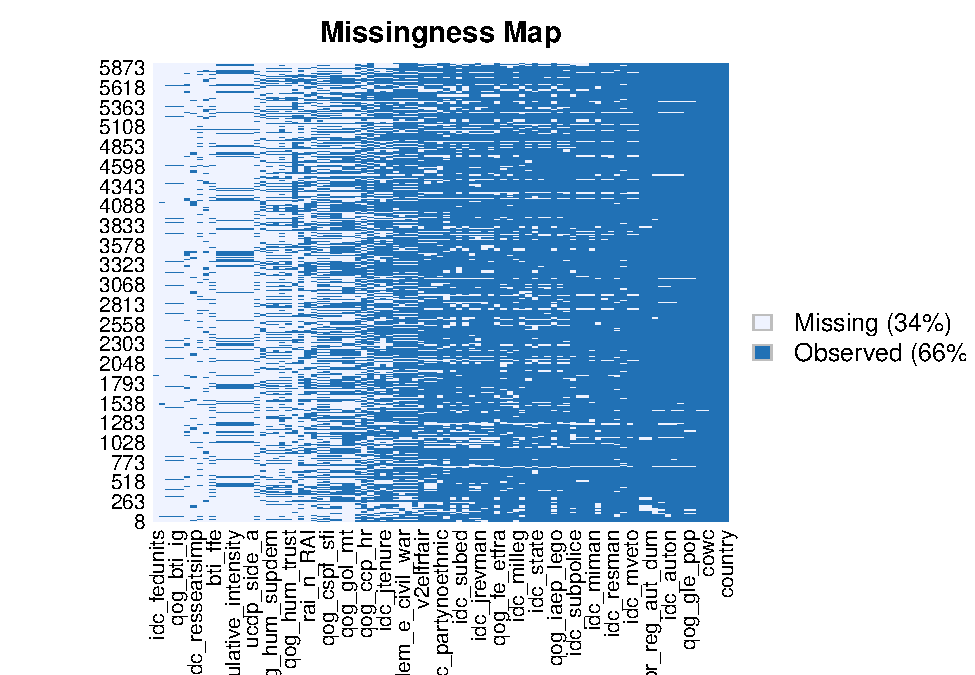
\includegraphics{01_tjbrailey_wrangle_data_files/figure-latex/unnamed-chunk-20-1.pdf}

\begin{Shaded}
\begin{Highlighting}[]
\KeywordTok{png}\NormalTok{(}\DataTypeTok{file =} \KeywordTok{paste0}\NormalTok{(here}\OperatorTok{::}\KeywordTok{here}\NormalTok{(), }\StringTok{"/vis/tjbrailey_psp_clean_missingness.png"}\NormalTok{),}
    \DataTypeTok{width =} \DecValTok{2000}\NormalTok{, }
    \DataTypeTok{height =} \DecValTok{1000}\NormalTok{)}
\NormalTok{Amelia}\OperatorTok{::}\KeywordTok{missmap}\NormalTok{(psp_add_bin)}
\end{Highlighting}
\end{Shaded}

\begin{verbatim}
## Warning: Unknown or uninitialised column: 'arguments'.
\end{verbatim}

\begin{verbatim}
## Warning: Unknown or uninitialised column: 'arguments'.
\end{verbatim}

\begin{verbatim}
## Warning: Unknown or uninitialised column: 'imputations'.
\end{verbatim}

\begin{Shaded}
\begin{Highlighting}[]
\KeywordTok{dev.off}\NormalTok{()}
\end{Highlighting}
\end{Shaded}

\begin{verbatim}
## pdf 
##   2
\end{verbatim}

\end{document}
